%\documentclass[manuscript,screen,anonymous,review]{acmart}
\documentclass[manuscript,review,anonymous]{acmart}
%\documentclass[manuscript,screen,anonymous,review,crop=false]{acmart}

\usepackage{enumitem}
\usepackage{csquotes}
\usepackage{graphicx}
\usepackage{tabularray}
\usepackage{tabularx}
\usepackage{multirow, makecell}
\usepackage{tabularx,array,booktabs}
\usepackage{array}
\usepackage{subcaption}
\usepackage{footnote}
\usepackage[export]{adjustbox}
%\usepackage[commandnameprefix=always, final,]{changes}
\usepackage{multicol}
\usepackage{import}
\usepackage{listings}

\usepackage[subpreambles=true]{standalone}

%\makeatletter
%\AddToHook{cmd/added/before}{\def\Changes@AuthorColor{blue}}
%\AddToHook{cmd/deleted/before}{\def\Changes@AuthorColor{red}}
%\AddToHook{cmd/replaced/before}{\def\Changes@AuthorColor{magenta}}
%\makeatother

\newcolumntype{P}[1]{>{\centering\arraybackslash}p{#1}}
\newcommand{\specialcell}[2][b]{\begin{tabular}[#1]{@{}c@{}}#2\end{tabular}}
\newcommand{\PreserveBackslash}[1]{\let\temp=\\#1\let\\=\temp}
\newcolumntype{C}[1]{>{\PreserveBackslash\centering}p{#1}}
\newcolumntype{R}[1]{>{\PreserveBackslash\raggedleft}p{#1}}
\newcolumntype{L}[1]{>{\PreserveBackslash\raggedright}p{#1}}

\usepackage{tikz}
\usetikzlibrary{automata, positioning, arrows, shapes.geometric,calc, shapes.multipart}

%%
%% \BibTeX command to typeset BibTeX logo in the docs
\AtBeginDocument{%
  \providecommand\BibTeX{{%
    Bib\TeX}}}

\setcopyright{acmlicensed}
\copyrightyear{2025}
\acmYear{2025}
\acmDOI{XXXXXXX.XXXXXXX}
%% These commands are for a PROCEEDINGS abstract or paper.
\acmConference[Conference acronym 'XX]{Make sure to enter the correct
  conference title from your rights confirmation email}{June 03--05,
  2018}{Woodstock, NY}
\acmISBN{978-1-4503-XXXX-X/2018/06}


\begin{document}

%\title{Towards a Visual FactSheet}
\title{Software Terms and Conditions: Know Before You Accept}

\author{SM Mozammal Hossain}
\affiliation{
	\institution{University of New Brunswick}
	\streetaddress{550 Windsor Street}
	\city{Fredericton}
	\state{NB}
	\country{Canada}
	\postcode{E3B 5A3}
}
\email{mozammal.hossain@unb.ca}

\author{Aaron Tabor}
\affiliation{
	\institution{University of New Brunswick}
	\streetaddress{550 Windsor Street}
	\city{Fredericton}
	\state{NB}
	\country{Canada}
	\postcode{E3B 5A3}
}
\email{Aaron.Tabor@unb.ca}

\author{Phil Munz}
\affiliation{
	\institution{TrojAI}
	\streetaddress{14 King St., Suite 102}
	\city{Saint John}
	\state{NB}
	\country{Canada}
	\postcode{E2L 1G2}
}
\email{phil.munz@troj.ai}

\author{Kenneth B. Kent}
\affiliation{
	\institution{University of New Brunswick}
	\streetaddress{550 Windsor Street}
	\city{Fredericton}
	\state{NB}
	\country{Canada}
	\postcode{E3B 5A3}
}
\email{ken@unb.ca}

\renewcommand{\shortauthors}{mozammal et al.}

\begin{abstract}

  In this AI driven era models are largely trained with data collected either via web crawling or offering free or paid online services. Long, text heavy, and hard-to-understand terms and conditions (T\&C) which are the conventional mechanism to inform and receive user consent showing their weaknesses. Several research has concluded that most users do not read and understand T\&C. This is not only because of the complexity of the T\&C but also number of online service one must use to perform their daily activities and they have little or no time to review those. We argue that users have been adequately informed about this data gathering or collection process through T\&C. Therefore, we propose an alternative approrach that summarizes T\&C using visual aid that makes hidden practices visible at a glance, highlights unknowns where policies are unclear or missing, and emphasize user impact in plain text.

  % How many online application a person uses in a day?

%  about the mutual benefits for both users and companies.

%  *   A **visual table** that maps **software terms** into clear categories: **data collection**, **data use**, **sharing**, **selling**, **retention**, and **ML risks**.
%
%  *   **Icons** replace dense text to show actions like **collect**, **process**, **share**, or **do not sell**.
%
%  *   **What it means**
%  *   Makes **hidden practices** visible at a glance.
%  *   Highlights **unknowns** (question marks) where policies are **unclear or missing**.
%  *   Emphasizes **user impact**, not legal wording.
%
%  *   **Why it’s included**
%  *   Demonstrates the **Visual FactSheet** concept in practice.
%  *   Shows how images can **improve understanding** over long text.
%
%  *   **How it fits the presentation**
%  *   Directly supports the **problem statement** about text-heavy terms.
%  *   Connects to the **user study** on image effectiveness.

%  \textbf{we won't be able to stop ai development. At best what we can do is to educate users for the their safety. it appears that people are not aware of that super intelligence can do in future.} This can be a paper idea.

\end{abstract}

%%
%% The code below is generated by the tool at http://dl.acm.org/ccs.cfm.
%% Please copy and paste the code instead of the example below.
%%
\begin{CCSXML}
<ccs2012>
 <concept>
  <concept_id>00000000.0000000.0000000</concept_id>
  <concept_desc>Do Not Use This Code, Generate the Correct Terms for Your Paper</concept_desc>
  <concept_significance>500</concept_significance>
 </concept>
 <concept>
  <concept_id>00000000.00000000.00000000</concept_id>
  <concept_desc>Do Not Use This Code, Generate the Correct Terms for Your Paper</concept_desc>
  <concept_significance>300</concept_significance>
 </concept>
 <concept>
  <concept_id>00000000.00000000.00000000</concept_id>
  <concept_desc>Do Not Use This Code, Generate the Correct Terms for Your Paper</concept_desc>
  <concept_significance>100</concept_significance>
 </concept>
 <concept>
  <concept_id>00000000.00000000.00000000</concept_id>
  <concept_desc>Do Not Use This Code, Generate the Correct Terms for Your Paper</concept_desc>
  <concept_significance>100</concept_significance>
 </concept>
</ccs2012>
\end{CCSXML}

\ccsdesc[500]{Do Not Use This Code~Generate the Correct Terms for Your Paper}
\ccsdesc[300]{Do Not Use This Code~Generate the Correct Terms for Your Paper}
\ccsdesc{Do Not Use This Code~Generate the Correct Terms for Your Paper}
\ccsdesc[100]{Do Not Use This Code~Generate the Correct Terms for Your Paper}

%%
%% Keywords. The author(s) should pick words that accurately describe
%% the work being presented. Separate the keywords with commas.
\keywords{Do, Not, Use, This, Code, Put, the, Correct, Terms, for,
  Your, Paper}

\received{20 February 2007}
\received[revised]{12 March 2009}
\received[accepted]{5 June 2009}

%%
%% This command processes the author and affiliation and title
%% information and builds the first part of the formatted document.
\maketitle

\section{Introduction}\label{intro}

	Machine learning (ML) assisted software services have become increasingly integrated into daily life. Although ML has been a prominent research area for many years, it initially struggled to demonstrate its superiority in solving commercially viable problems, which led to slower adoption of ML technology. Limitations in ML algorithms, development tools, hardware resources, and the availability of training data further contributed to this slow commercial uptake. Over the past decade, ML has evolved dramatically and has become a core component of many automated services, e.g., answering citizen inquiries related to unemployment benefits, welfare programs, and other public services \cite{10.1093/ppmgov/gvaf013}. Extensive research efforts have resulted in the development of numerous ML strategies, techniques, and algorithms. With advancements in Deep Learning (DL), Natural Language Processing (NLP), and most recently, Large Language Models (LLMs), ML has proven its ability to tackle complex problems with commercial value \cite{li_impact_2023} \cite{pugliese_machine_2021}. As a result, leading corporations such as Microsoft, Google, IBM, Amazon, and others have begun investing heavily integrate ML into their products. Although Google and Amazon experimented with and incorporated ML techniques in their products in a limited scope as early as 2014, recent breakthroughs in DL and LLMs particularly in image recognition and language processing have accelerated their large scale commercial adoption to improve their search results and product recommendations. Other influential players, e.g., IBM, Meta, and many more have followed similar adoption paths. Today, it is difficult to find mid-sized or large companies offering products without incorporating some form of ML capability.

	ML assisted systems require large volumes of data for training. Both established and emerging companies interested in developing ML based services or applications have been collecting data, actively or passively, for extended periods. By offering free services such as search engines, social media, and e-commerce platforms, companies routinely collect user data. Loyalty programs are another mechanism used by retailers to gather consumer information. These data are often used for user profiling, personalized product recommendations, and targeted advertising. The process of data collection continues to accelerate. At present, approximately 19.8 billion Internet of Things (IoT) devices are connected to the internet, generating 2.5 quintillion bytes of data daily \cite{statistica_2} \cite{seedscientific}. This growth is projected to continue, with expectations that by 2034 40.6 billion IoT devices will be connected globally and will collectively produce 527.5 zettabytes of data annually \cite{statistica_1} \cite{statistica_2}.

	Prior to the introduction of the General Data Protection Regulation (GDPR) in 2016, organizations faced limited regulatory oversight regarding how data were collected and used \cite{GDPR2016a}. A similar lack of oversight also applied to ML model development until the emergence of formal AI governance policies. GDPR, introduced by the European Union (EU), enforces strict requirements related to data collection, processing, ownership, retention, and usage. These regulations present significant challenges for organizations involved in the development and deployment of ML based systems. Despite these regulatory advances, publicly available information about how ML models underlying AIS are built, trained, and evaluated remains limited. As a result, such systems are often criticized for a lack of transparency, commonly referred to as the “black box” problem, where the reasoning behind decisions or recommendations is unclear \cite{app15020672} \cite{10.2478} \cite{JSSv036i11}. While companies often rely on traditional, text based “Terms and Conditions” or “Terms of Use” agreements to disclose data collection and usage practices, these documents are widely regarded as ineffective at conveying meaningful information to users \cite{buttarelli_we_2019}. In this paper, we propose a documentation framework designed to better serve the needs of all stakeholders by improving transparency, interpretability, and informed user decision making.

\section{Literature Review}\label{liturea_review}

	We investigated existing contribution in three criteria. At the beginning, we wanted to understand complexity of the T\&C, whether they understand what was in those T\&C, and how users are reacting to those. Secondly, we investigated what efforts were made in the RAI domain to ensure its goals. Finally, we investigated the existing work of using image based documentation framework to assist user to understand complex, tex-heavy T\&C. Our findings of each criteria are discussed in next three sub-sections.

\subsection{Complexity of T\&C}

	In today's ML driven era, especially with the rise of generative AI applications, users should be informed, or service providers should disclose, details about the underlying AI technology, data collection, processing, privacy practices, and data usage in a way that is easy to understand. Unfortunately, text-based legal agreements mentioned in Section \ref{intro} are the only approach currently used. A Deloitte survey in 2017 revealed that 91\% of 2,000 U.S. participants accepted "Terms and Conditions" or "Terms of Use" agreements without reading them. The same survey found that this trend was even stronger among individuals aged 18–38, with 97\% agreeing without reading \cite{cakebread_youre_2014}. Similarly, Obar et al. conducted a study using a fictitious social networking platform with two documents: a privacy policy (PP) and terms of service (TOS). They estimated that reading the PP and TOS would take 29–32 and 15–17 minutes, respectively, yet participants spent only 73 and 51 seconds before agreeing. Among 543 participants, mostly undergraduate students from a large communication class at a public university in the eastern U.S., 97\% agreed to the PP and 93\% to the TOS \cite{obar_biggest_2016}.

	For English-speaking adults, the average oral reading rate is 183 words per minute (wpm), and the silent reading rate can be up to 280-320 wpm \cite{obar_biggest_2016}\cite{brysbaert_how_2019}. Table \ref{tab:lincenseLength} shows the word count of license agreements for some of the most popular and widely used applications or services. It is surprising to observe that some of the most popular free service providers, i.e., Meta, Tinder, Microsoft, etc., crafted their license agreements in such a way that, for a regular user, it could take 14.4 to 63.5 minutes to read them. Table \ref{tab:lincenseLength} results were based on 2020 data. We assume that most users did not spend much time reviewing and understanding their rights, responsibilities, data collection, and possible usage before agreeing to the terms. Our assumption is based on the survey findings conducted by Obar et al., where participants agreed to share their data with the United States national security agency and their employer, and provided their first-born child as payment for social networking service access \cite{obar_biggest_2016}. From the above discussion, we conclude that traditional, text-heavy, lengthy legal agreements between service providers and users are inadequate in delivering appropriate messages to their audience. We advocate for a clear, easily understandable communication mechanism or framework for AI system users, explaining their rights and responsibilities.

	\begin{table}[h!]
		\centering
		\input{table/License.tex}
		\caption{License Length and Reading Time \cite{lepan_visualizing_2020}}
		\label{tab:lincenseLength}
	\end{table}

\subsection{Literacy Level}

	OECD
	The SMOG Formula

\subsection{RAI Initiative}

	A Fact Sheet is defined as "a single-page or other brief document presenting facts relevant to a specific issue" \cite{oxford_university_press_fact_nodate}. In ML development, a \enquote{Fact Sheet}, also referred to as \enquote{FactSheets} (FS), is a documentation framework designed to support responsible AI (RAI) practices \cite{arnold_factsheets_2018}. We consider it the cornerstone of all governance tools. Originally introduced by Arnold et al., the FS framework aims to promote transparency and trustworthiness in ML services and applications for auditors and developers. This trust is achieved by documenting every stage of the ML development lifecycle \cite{arnold_factsheets_2018}. Acting as a repository for outputs from RAI tools such as bias detection and mitigation, explainability, robustness, performance, etc., the FS extends traditional software documentation with a strict focus on AI development. Hind et al. noted that the FS proposed by Arnold et al. can serve multiple purposes for different stakeholders \cite{hind_experiences_2020}, though we believe end users were overlooked in their design. Other initiatives include Michell et al.'s "Model Cards", which emphasize reporting performance, use cases, and fairness, and Gebru et al.'s "Datasheets for Datasets", a comprehensive data-focused document answering 57 questions on data collection, processing, and usage \cite{mitchell_model_2019} \cite{gebru_datasheets_2021}. Both Arnold et al. and Hind et al. adopted a question-and-answer methodology targeting developers, data scientists, technical stakeholders, and testers but excluded end users \cite{arnold_factsheets_2018} \cite{hind_experiences_2020}. Similarly, Kasia et al.'s CLeAR framework supports AI practitioners and policymakers \cite{chmielinski2024the}, yet fails to address end users' needs. In summary, FSs are vital throughout an ML project, from development to deployment and beyond. We conclude that researchers' contributions, discussed above, offer a robust approach for personnel engaged in ML development.

\subsection{Use of Image}

	Zhang et al. introduced privacy nutrition labels for mobile applications offering a limited subset of information, their approach is not fully applicable to ML assisted software \cite{298912}. Our proposed VFS builds upon and partially resembles Zhang et al.'s contribution but is specifically tailored for ML assisted software.

\subsection{Discussion}
	Currently, there is no standardized framework for documenting key aspects of ML models, i.e., how training data is collected and processed or how model performance is evaluated. FS, \enquote{Model Cards}, \enquote{Datasheets for Datasets}, and \enquote{CLeAR} initiatives represent significant steps toward achieving RAI objectives. However, these efforts have largely overlooked the importance of involving end users. Moreover, they lack a unified template for capturing all relevant ML details. While Arnold et al. proposed a project-specific FS template, we argue that this should become a universal standard \cite{arnold_factsheets_2018}. Similarly, Hind et al. and Arnold et al. anticipated that FS would serve multiple user groups but failed to classify these groups or provide clear guidelines on which ML details should be included for different FS types \cite{arnold_factsheets_2018} \cite{hind_experiences_2020}.

	In this paper, we propose a visual documentation framework, i.e., \enquote{Visual FactSheet} (VFS), designed for non-technical users.

\section{Proposed Work}

	Governance in AI is an evolving discipline that includes key principles such as fairness, bias mitigation, explainability, robustness, causal inference, and privacy. Understanding the system's capabilities and limitations is essential for AIS users. A FS aims to provide users with all necessary information to make informed decisions. While FS is widely acknowledged as an important tool advancing RAI when implemented correctly, the term is often ambiguous, overused, and misunderstood. To ensure clarity and effectiveness, FS must have a well-defined, comprehensive, and actionable structure aligned with RAI principles. Traditionally, an FS may take the form of a lengthy, text-heavy document detailing relevant attributes across multiple sections. However, we argue that a single, exhaustive FS meets the needs of all audiences. Hence, we propose FS be tailored for distinct user groups instead of a long generic FS. We presented our work on FS user identification in Section \ref{userGroup.}.

	At the age of interactive information systems, digital icons or pictorial signs play an important role in conveying information quickly in contrast to the use of text. Universally accepted icons can also break written language and cultural barriers, and convey large amounts of information efficiently and concisely \cite{COLLAUD2022102290} \cite{doi:10.1177/2041669518780807} \cite{doi:10.1177/2041669518780807}. In addition, the human brain can process and retain information more quickly when presented visually. Potter et al. conducted an experiment in 2014 that revealed humans can process an entire image in 13 milliseconds, even if they have not seen the image before \cite{Potter2014-ih}. Based on the information presented in Sections \ref{intro} and \ref{liturea_review}, and the discussion above, we propose utilizing visual aids, i.e., images in FS for conveying necessary information to end users prior to using any AIS. Our hypothesis is that our proposed VFS will eliminate or reduce constraints that a text-heavy FS brings. To examine our hypothesis, we prepared VFS for two popular AIS using their Terms and Conditions that are presented in Section \ref{example} Figure \ref{fig:ChatGPT} and in Appendix \ref{appendix:a} Figure \ref{fig:Equifax}. In order to evaluate our proposed hypothesis, we conducted a user survey involving xx participants and presented our findings in Section \ref{surveyResult}.

\section{Methodology}\label{VFS_Methodology}
	To design our VFS framework, we utilized the methodology proposed by Venable, J., originated in the Design Science Research (DSR) for developing information systems, as shown in Figure \ref{fig:designscienceframework} \cite{Venable2006TheRO}. The core of this methodology is technology innovation (TI) that relies on three other tightly coupled, bi-directional components. Through the TI phase, a technology or method is created or enhanced, and we utilize this component to enhance the FS documentation process by introducing visual aids for enabling quick information transfer and clarity. We followed the image selection strategy discussed later in this Section. We evaluated our proposed VFS through a user survey and rectified our solution following the problem diagnosis and technology evaluation components of the DSR methodology.

	\begin{figure}[h!]
		\centering
		\scalebox{0.90}[1]{%pdflatex VFS.tex
%pdftoppm -png VFS.pdf output

\documentclass{standalone}


%\usepackage{graphicx}
\usepackage{tikz}
\usepackage{geometry}
\usetikzlibrary{automata, positioning, arrows, shapes.geometric,calc, shapes.multipart}
%\geometry{letterpaper}

%\newcommand{\specialcell}[2][b]{\begin{tabular}[#1]{@{}c@{}}#2\end{tabular}}

\begin{document}
	
	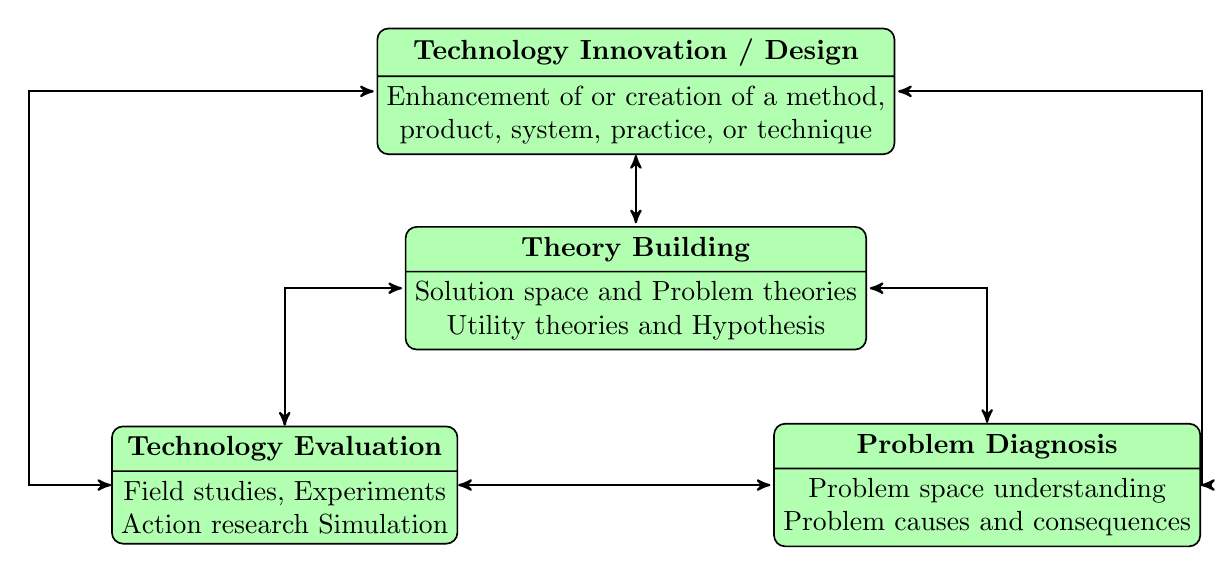
\begin{tikzpicture}[scale=0.50, ->, >=stealth', shorten >=1pt, node distance=6cm, semithick,
		every state/.style={rectangle, text centered, rounded corners, black, draw=black, fill=green!30, minimum width=2cm,minimum height=1.2cm,}]
		
		\node[state] (TechEval) [align=center, rectangle split, rectangle split parts=2] 
		{\textbf{Technology Evaluation} \nodepart{second} Field studies, Experiments \\ Action research Simulation};
		
		\node[state] (ProbDiag) [right=4cm of TechEval, align=center, rectangle split, rectangle split parts=2] 
		{\textbf{Problem Diagnosis} \nodepart{second} Problem space understanding \\ Problem causes and consequences};
		
		\node[state] (TechInnovDesg) [yshift=5cm, align=center, rectangle split, rectangle split parts=2] at ($(TechEval)!0.5!(ProbDiag)$)
		{\textbf{Technology Innovation / Design} \nodepart{second} Enhancement of or creation of a method, \\ product, system, practice, or technique};
		
		\node[state] (TheoryBld) [below of=TechInnovDesg, yshift=3.5cm, align=center, rectangle split, rectangle split parts=2]
		{\textbf{Theory Building} \nodepart{second} Solution space and Problem theories \\ Utility theories and Hypothesis};
		
		\draw[<->, thick] (TechInnovDesg.south) -- (TheoryBld.north);
		\draw[<->, thick] (TechEval.east) -- (ProbDiag.west);
		\draw[<->, thick] (TechEval.west) -| (-6.5,1.5) |- (TechInnovDesg.west);
		\draw[<->, thick] (TechEval.north) |- (TheoryBld.west);
		\draw[<->, thick] (ProbDiag.east) -| (23.3,1.5) |- (TechInnovDesg.east);
		\draw[<->, thick] (ProbDiag.north) |- (TheoryBld.east);
		
	\end{tikzpicture}

\end{document}

}
		\caption{An activity framework for design science research \cite{Kuechler01102008}.}
		\label{fig:designscienceframework}
	\end{figure}

\subsection{Participant Enrollment}
	We have taken several methods to recruit participants. Our primary strategy was to take advantage of UNB media communication, campus wide physical poster and email, use of social media. We also make initiatives through presentation in an classroom and research exposition setting. Participants were not compensated either Monetary or any other form of compensation. Since the was anonymous in nature, we were unable to identify their country of origin.

	Although we identified several user groups, this paper concentrates exclusively on the End User group. This choice reflects our intent to prioritize the ML data producer rather than the data consumer. The remaining user groups we identified exhibit a high degree of specialization, and recruitment from these groups would require more time compared to end users, as Khalid and Brown showed that domain-specific participant recruitment often encounters challenges such as locating eligible individuals, communication delays, establishing appropriate screening criteria, and addressing trust-related concerns \cite{10714565}.

\subsection{VFS Design}
	While designing our VFS template, we followed a risk-based approach. For ML development, there are mainly two types of risks: data-level and model-level risks. Data risk encapsulates data bias, shift, adversarial attack, etc., while model-level risk includes accuracy, uncertainty, etc. \cite{ZHANG2022113800}. Instead of treating them separately, we followed a hybrid approach, combining the ML model's data bias and fairness risk into one, accuracy solely for the model, and leaving a wide range for any other risk the provider may consider informing its users of. We propose the below components in a VFS that we consider most important for end-users: \enquote{Purpose}, \enquote{Data Collection}, \enquote{Data Processing}, \enquote{Data Sharing}, \enquote{Data Selling}, \enquote{Data Retention}, \enquote{Accuracy, Fairness}, and \enquote{Potential Risk}.

\subsection{Image Selection }
	While appropriate images can transfer information at lightning speed, increasing the completeness and readability of documents, inappropriate ones may result in poor results, especially in e-commerce, where icon or image selection affects click-through rate \cite{Hyun2022} \cite{10.1145/3543873.3584646}. Although in this work, we are not going to design any images for our proposed VFS, we will instead use the most commonly used, publicly available images. We need to select images carefully with the intention of avoiding misinterpretation. We aligned our image selection strategy with the image design standards discussed by Collaud et al. These are \enquote{access to meaning, familiarity, visual complexity, and aesthetic appeal} \cite{COLLAUD2022102290}.

\subsection{Ethical Considerations}
	To evaluate our Visual FactSheet (VFS) hypothesis that visual representations can improve transparency around data collection when using free software services such as social media, we developed an end user focused online survey distributed through multiple channels, including social media. The survey, titled \enquote{Towards a Visual FactSheet for Software Terms and Conditions Agreements}, received approval from the University of New Brunswick (UNB) Faculty of Computer Science and the UNB Research Ethics Board (REB), under file number \textbf{REB 2026‑030}. The survey aims to engage participants not only from the UNB community (students, faculty, and staff) but also from external audiences, including our industry partner, TrojAI. A subsequent modification request was submitted to the UNB REB to include a physical poster to support participant recruitment, which was also approved.

	It also reassures them that the survey adheres to the ethical guidelines established by the Tri Council Policy Statement of Canada, as enforced by the UNB Research Ethics Board (REB). Additionally, this section includes contact information for the responsible personnel should participants require further details or have any concerns. At the end of the section, participants are asked to provide their consent, which is recorded in accordance with REB requirements. No PII is collected or used in this survey. The project also measures participants’ subjective workload using the NASA Task Load Index (NASA TLX)\cite{hart1988development}.

\section{Components of Visual FactSheet}\label{ComponentsVFS}

	\enquote{A Picture Is Worth a Thousand Words} \cite{sullivan_picture_2017}. Visual depictions of complex agreements not only provide clarity of the content but also can enhance a nontechnical person's decision-making process \cite{suters_emergence_2023, kim_impact_2021}. While the use of visual depictions over text-heavy content makes it easier to understand product instructions for many companies, it is uncommon to use the same strategy for capturing a user's response of proper understanding of the license agreement, despite their possible effectiveness for improving information quality, credibility, and enhancing the decision-making process \cite{kim_impact_2021}. We expect a VFS will be a useful approach to inform license information pictorially.

	Data is the fuel for any ML model. Training data acts as an input for the ML model and dictates how it will perform while providing recommendations. There is a common notion that the more data an ML model is trained on, the more accurately it will perform \cite{nield2022essential}. Hence, data has become the new currency in today's interconnected world \cite{Gates:2014:DNC:2683467.2683477}. Due to this reason, we concluded users should know what data they are sharing and how the provided data will be retained, processed, and shared.

	A VFS should begin by clearly stating the purpose of the AIS service, including an example problem and how the service addresses it. Users must be informed about the types of data the AIS provider may collect during usage. While providing examples of collected data is optional, it is strongly recommended. At the very least, the provider should confirm whether data collection occurs with a clear \enquote{Yes} or \enquote{No}. If data collection is confirmed, the provider must explain why the data is collected and how it will be used in the future. Additionally, the provider should specify measures taken to ensure that no PII is included, again at least with a simple \enquote{Yes} or \enquote{No} acknowledgment.

	When user data is collected and processed, providers must disclose their data retention policies and explain how the data will be securely destroyed once the retention period ends. AIS providers frequently share collected data with affiliates, government agencies (including law enforcement), and other third-party AIS providers. In the event of business transfers, ownership of this data may also change. Providers should clearly identify all recipients of the data and specify whether it will be shared in raw or processed form.

	Regardless of whether the service is free or paid, AIS providers must demonstrate the effectiveness and value of their offerings. For AIS solutions, the accuracy of underlying machine learning models is a critical metric. Given ongoing concerns about bias and fairness, providers should inform users about the impartiality of their services, including reported accuracy, fairness, and bias percentiles. Finally, AIS services may carry inherent risks. Growing concerns include adversarial attacks on machine learning models, as well as threats such as data poisoning, model theft, and hijacking. Service providers must recognize these vulnerabilities and clearly outline the measures implemented to mitigate or prevent them.

\subsection{VFS Example}\label{example}

	We illustrate VFS with two case studies: a free service (ChatGPT) and a paid service (Equifax), as they are among the most widely used AI platforms. We use the VFS framework to visually analyze the data these services collect, process, sell, and share. Additionally to assess the transparency of their machine learning models which is the core of their functionality.

	ChatGPT, developed by OpenAI and launched in November 2022, is a chatbot built on LLM architecture to enable natural language processing and human-like conversations for task assistance and information retrieval \cite{ortiz_what_nodate}. In our study, we reviewed its \enquote{Privacy Policy} and created the VFS shown in Figure \ref{fig:ChatGPT}, with explanatory legends for the icons in Figure \ref{fig:VSLegends}. Figure \ref{fig:ChatGPT} illustrates the categories of data collected by OpenAI during user interactions with ChatGPT, including personal details, social media information, device identifiers, and communication content. Realtime analytics are applied to these data to enhance user experience. Figure \ref{fig:ChatGPT} also depicts how OpenAI processes, shares, and retains user data indefinitely. These data are utilized for research, product development, and service improvement, and may be shared with government agencies, third-party vendors, and affiliated entities \cite{openai_privacy_2023}. Despite ChatGPT’s foundation in LLM technology, no public documentation exists regarding its architecture, accuracy, associated risks, or fairness and bias in the training data.

	\begin{figure}[!t]
		\begin{minipage}{0.48\textwidth}
			\scalebox{0.6}{%pdflatex VFS.tex
%pdftoppm -png VFS.pdf output

\documentclass{standalone}

\usepackage{graphicx}
\usepackage[export]{adjustbox}
\usepackage{multirow, multicol}
\graphicspath{{C:/MyFolder/Working_Papers/Working_Papers/facct_conf/}}
%\newcommand{\specialcell}[2][b]{\begin{tabular}[#1]{@{}c@{}}#2\end{tabular}}

\begin{document}

	\begin{tabular}{|c|c|c|}
		\hline
%		\multicolumn{3}{|c|}{\specialcell{ChatGPT is an LLM based chatbot that processes natural language \\ to provide human-like conversational assistance.}} \\ [0.5ex]
%		\hline
		\specialcell{\\[-8pt] \textbf{\large {Group}}} & \textbf{\large {Action}} & \textbf{\large {Activity}} \\ [0.5ex]
		\hline
		\multirow{2}{*}{\rotatebox[origin=rc]{90}{\textbf{General}}}
		& \specialcell{You Must \\ be} & \specialcell{\\[-8pt]
			
\includegraphics[width=12mm, valign=mc]{images/13_modified}
		}\\[0.5ex]
		\cline{2-3}
		& \specialcell{You Must \\ Provide} & \specialcell{\\[-8pt]
			
\includegraphics[width=12mm, valign=mc]{images/accurate_modified} }\\[0.5ex]
		\cline{2-3}
		\hline
		\multirow{4}{*}{\rotatebox[origin=rc]{90}{\textbf{User Data}}} &
		\specialcell{We Collect \\ Your Data} & \specialcell{\\[-8pt]
			
\includegraphics[width=12mm, valign=mc]{images/socialmedia_modified}
			
\includegraphics[width=12mm, valign=mc]{images/personalinformation_modified}
			
\includegraphics[width=12mm, valign=mc]{images/selfie_modified}
			
\includegraphics[width=12mm, valign=mc]{images/smartphone_modified}
			
\includegraphics[width=12mm, valign=mc]{images/httpcookie_modified}
			%				
\includegraphics[width=12mm, valign=mc]{images/analytics} \hspace{0.4cm}
			
\includegraphics[width=12mm, valign=mc]{images/location_modified}
			
\includegraphics[width=12mm, valign=mc]{images/payment_modified} } \\ [0.5ex]
		\cline{2-3} &
		\specialcell{We Process \\ Data For} & \specialcell{\\[-8pt]
			
\includegraphics[width=12mm, valign=mc]{images/gear_modified}
			
\includegraphics[width=12mm, valign=mc]{images/research_modified}
			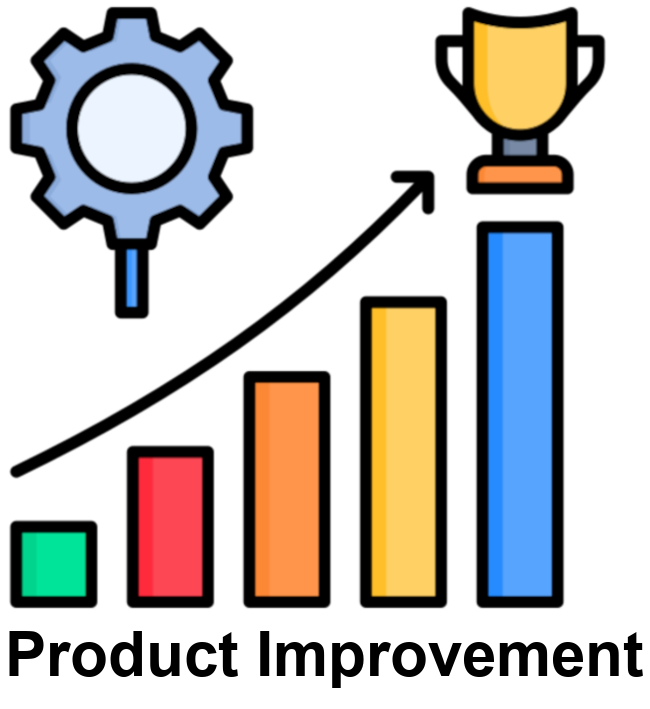
\includegraphics[width=12mm, valign=mc]{images/improvement_modified}
			
\includegraphics[width=12mm, valign=mc]{images/product-development_modified} } \\ [0.5ex]
		\cline{2-3} &
		\specialcell{We Share \\ Data With}  & \specialcell{\\[-8pt]
			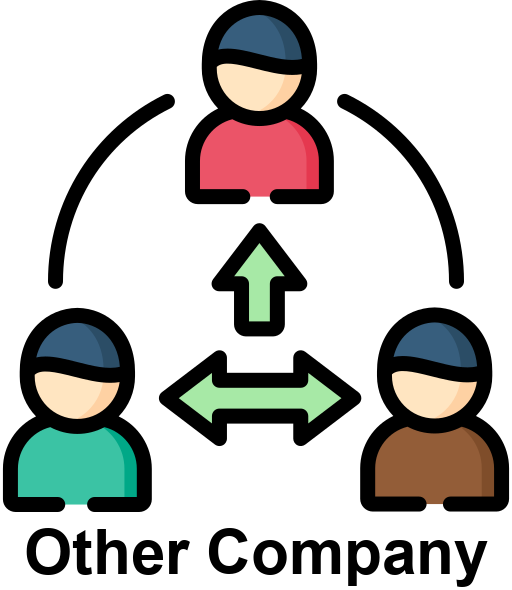
\includegraphics[width=12mm, valign=mc]{images/thirdparty_modified}
			
\includegraphics[width=12mm, valign=mc]{images/policeman_modified}
			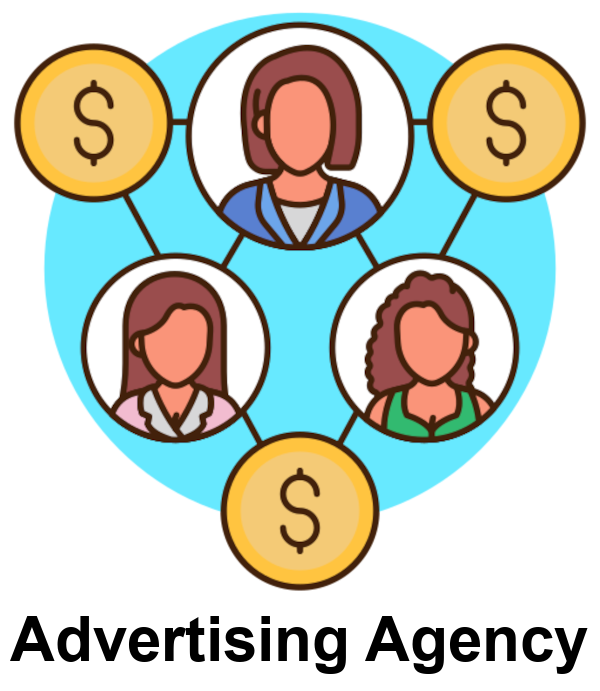
\includegraphics[width=12mm, valign=mc]{images/affiliate_modified}
			
\includegraphics[width=12mm, valign=mc]{images/payment_modified} } \\ [0.5ex]
		\cline{2-3} &
		\specialcell{We Sell \\ Data To} & \specialcell{\\[-8pt]
			
\includegraphics[width=12mm, valign=mc]{images/no-sale_modified} } \\ [0.5ex]
		\cline{2-3} &
		\specialcell{Retention \\ Period} & \specialcell{\\[-8pt]
			
\includegraphics[width=12mm, valign=mc]{images/unknown_modified} } \\ [0.5ex]
		\hline
		\multirow{4}{*}{\rotatebox[origin=rc]{90}{\textbf{Machine Learning}}} &
		Accuracy & \specialcell{\\[-8pt]
			
\includegraphics[width=12mm, valign=mc]{images/unknown_modified} } \\ [0.5ex]
		\cline{2-3} &
		\specialcell{Fairness \\ and Bias} & \specialcell{\\[-8pt]
			
\includegraphics[width=12mm, valign=mc]{images/unknown_modified} } \\ [0.5ex]
		\cline{2-3} &
		\specialcell{Potential \\ Risk} & \specialcell{\\[-8pt]
			
\includegraphics[width=12mm, valign=mc]{images/unknown_modified} } \\ [0.5ex]
		\hline
		\multicolumn{3}{|c|}{\specialcell{\\[-8pt]\textbf{Source:} All images were downloaded from Flaticon.com}} \\ [0.5ex]
		\hline

	\end{tabular}

\end{document}

}
			\caption{Visual FactSheet for ChatGPT }
			\label{fig:ChatGPT}
		\end{minipage}
		\hfill % Adds spacing between the two
		\begin{minipage}{0.48\textwidth}
			\scalebox{0.6}{%pdflatex VFS.tex
%pdftoppm -png VFS.pdf output

\documentclass{standalone}

\usepackage{graphicx}
\usepackage[export]{adjustbox}
\usepackage{multirow, multicol}

%\newcommand{\specialcell}[2][b]{\begin{tabular}[#1]{@{}c@{}}#2\end{tabular}}

\begin{document}

	\begin{tabular}{|c|c|c|}
%		\hline
%		\multicolumn{3}{|c|}{\specialcell{\\[-8pt] Equifax is a credit bureau providing online access to credit score and report, \\ credit monitoring, alerts and identity theft protection.}} \\ [0.5ex]
		\hline
		\specialcell{\textbf{\large {Group}}} & \textbf{\large {Action}} & \textbf{\large {Activity}} \\ [0.5ex]
		\hline
		\multirow{2}{*}{\rotatebox[origin=rc]{90}{\textbf{General}}}
		& \specialcell{You Must \\ be} & \specialcell{\\[-8pt]
			
\includegraphics[width=12mm, valign=mc]{images/18_modified}
		}\\[0.5ex]
		\cline{2-3}
		& \specialcell{You Must \\ Provide} & \specialcell{\\[-8pt]
			
\includegraphics[width=12mm, valign=mc]{images/accurate_modified} }\\[0.5ex]
		\cline{2-3}
		\hline
		\multirow{4}{*}{\rotatebox[origin=rc]{90}{\textbf{User Data}}} &
		\specialcell{We Collect \\ Your Data} & \specialcell{\\[-8pt]
			
\includegraphics[width=12mm, valign=mc]{images/id_modified} \hspace{0.2cm}
			
\includegraphics[width=12mm, valign=mc]{images/personalinformation_modified} \hspace{0.2cm}
			
\includegraphics[width=12mm, valign=mc]{images/selfie_modified}
			
\includegraphics[width=12mm, valign=mc]{images/smartphone_modified}
			
\includegraphics[width=12mm, valign=mc]{images/httpcookie_modified}
			
\includegraphics[width=12mm, valign=mc]{images/location_modified} \\
			
\includegraphics[width=12mm, valign=mc]{images/payment_modified}
			
\includegraphics[width=12mm, valign=mc]{images/monitoring_modified}
			
\includegraphics[width=12mm, valign=mc]{images/shopping-cart_modified}} \\ [0.5ex]
		\cline{2-3} &
		\specialcell{We Process \\ Data For} & \specialcell{\\[-8pt]
			
\includegraphics[width=12mm, valign=mc]{images/gear_modified}
			
\includegraphics[width=12mm, valign=mc]{images/research_modified}
			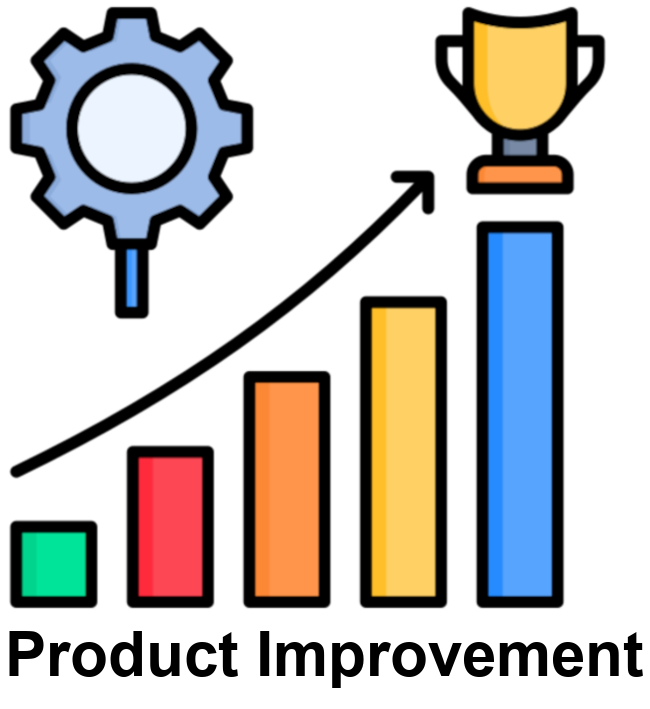
\includegraphics[width=12mm, valign=mc]{images/improvement_modified}
			
\includegraphics[width=12mm, valign=mc]{images/product-development_modified} } \\ [0.5ex]
		\cline{2-3} &
		\specialcell{We Share \\ Data With}  & \specialcell{\\[-8pt]
			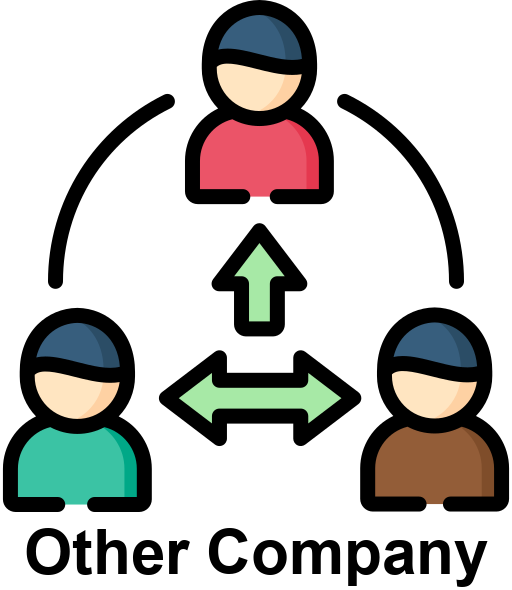
\includegraphics[width=12mm, valign=mc]{images/thirdparty_modified}
			
\includegraphics[width=12mm, valign=mc]{images/policeman_modified}
			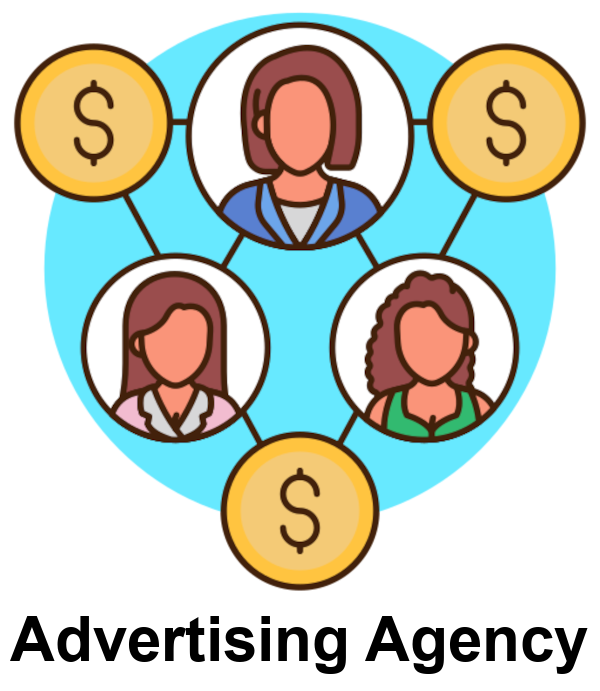
\includegraphics[width=12mm, valign=mc]{images/affiliate_modified}
			
\includegraphics[width=12mm, valign=mc]{images/payment_modified} } \\ [0.5ex]
		\cline{2-3} &
		\specialcell{We Sell \\ Data To} & \specialcell{\\[-8pt]
			
\includegraphics[width=12mm, valign=mc]{images/job_modified}
			
\includegraphics[width=12mm, valign=mc]{images/insurance-company_modified}
			
\includegraphics[width=12mm, valign=mc]{images/policeman_modified}} \\ [0.5ex]
		\cline{2-3} &
		\specialcell{Retention \\ Period} & \specialcell{\\[-8pt]
			
\includegraphics[width=12mm, valign=mc]{images/unknown_modified} } \\ [0.5ex]
		\hline
		\multirow{4}{*}{\rotatebox[origin=rc]{90}{\textbf{Machine Learning}}} &
		Accuracy & \specialcell{\\[-8pt]
			
\includegraphics[width=12mm, valign=mc]{images/unknown_modified} } \\ [0.5ex]
		\cline{2-3} &
		\specialcell{Fairness \\ and Bias} & \specialcell{\\[-8pt]
			
\includegraphics[width=12mm, valign=mc]{images/unknown_modified} } \\ [0.5ex]
		\cline{2-3} &
		\specialcell{Potential \\ Risk} & \specialcell{\\[-8pt]
			
\includegraphics[width=12mm, valign=mc]{images/unknown_modified} } \\ [0.5ex]
		\hline
		\multicolumn{3}{|c|}{\specialcell{\\[-8pt]\textbf{Source:} All images were downloaded from Flaticon.com}} \\ [0.5ex]
		\hline
	\end{tabular}

\end{document}

}
			\caption{Visual FactSheet for Equifax }
			\label{fig:Equifax}
		\end{minipage}
	\end{figure}

%	\begin{figure}[h!]
%		\centering
%		%pdflatex VFS.tex
%pdftoppm -png VFS.pdf output

\documentclass{standalone}

\usepackage{graphicx}
\usepackage[export]{adjustbox}
\usepackage{multirow, multicol}
\graphicspath{{C:/MyFolder/Working_Papers/Working_Papers/facct_conf/}}
%\newcommand{\specialcell}[2][b]{\begin{tabular}[#1]{@{}c@{}}#2\end{tabular}}

\begin{document}

	\begin{tabular}{|c|c|c|}
		\hline
%		\multicolumn{3}{|c|}{\specialcell{ChatGPT is an LLM based chatbot that processes natural language \\ to provide human-like conversational assistance.}} \\ [0.5ex]
%		\hline
		\specialcell{\\[-8pt] \textbf{\large {Group}}} & \textbf{\large {Action}} & \textbf{\large {Activity}} \\ [0.5ex]
		\hline
		\multirow{2}{*}{\rotatebox[origin=rc]{90}{\textbf{General}}}
		& \specialcell{You Must \\ be} & \specialcell{\\[-8pt]
			
\includegraphics[width=12mm, valign=mc]{images/13_modified}
		}\\[0.5ex]
		\cline{2-3}
		& \specialcell{You Must \\ Provide} & \specialcell{\\[-8pt]
			
\includegraphics[width=12mm, valign=mc]{images/accurate_modified} }\\[0.5ex]
		\cline{2-3}
		\hline
		\multirow{4}{*}{\rotatebox[origin=rc]{90}{\textbf{User Data}}} &
		\specialcell{We Collect \\ Your Data} & \specialcell{\\[-8pt]
			
\includegraphics[width=12mm, valign=mc]{images/socialmedia_modified}
			
\includegraphics[width=12mm, valign=mc]{images/personalinformation_modified}
			
\includegraphics[width=12mm, valign=mc]{images/selfie_modified}
			
\includegraphics[width=12mm, valign=mc]{images/smartphone_modified}
			
\includegraphics[width=12mm, valign=mc]{images/httpcookie_modified}
			%				
\includegraphics[width=12mm, valign=mc]{images/analytics} \hspace{0.4cm}
			
\includegraphics[width=12mm, valign=mc]{images/location_modified}
			
\includegraphics[width=12mm, valign=mc]{images/payment_modified} } \\ [0.5ex]
		\cline{2-3} &
		\specialcell{We Process \\ Data For} & \specialcell{\\[-8pt]
			
\includegraphics[width=12mm, valign=mc]{images/gear_modified}
			
\includegraphics[width=12mm, valign=mc]{images/research_modified}
			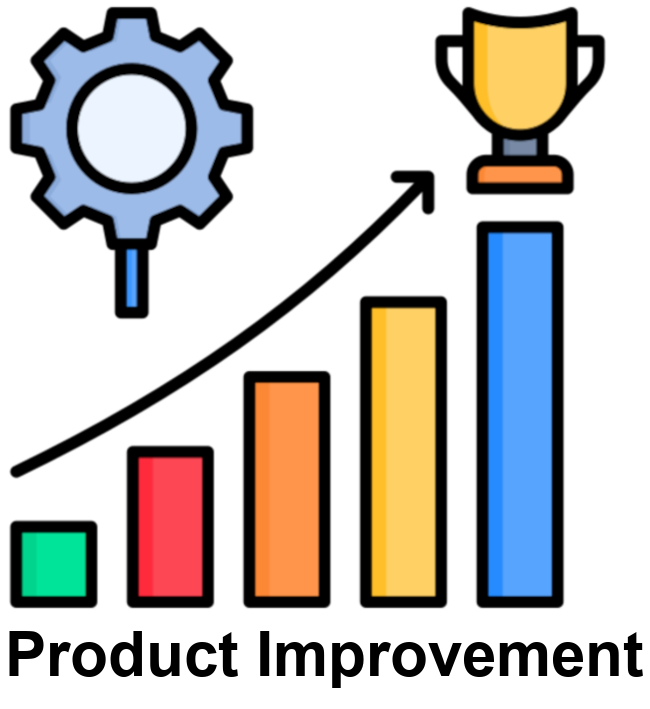
\includegraphics[width=12mm, valign=mc]{images/improvement_modified}
			
\includegraphics[width=12mm, valign=mc]{images/product-development_modified} } \\ [0.5ex]
		\cline{2-3} &
		\specialcell{We Share \\ Data With}  & \specialcell{\\[-8pt]
			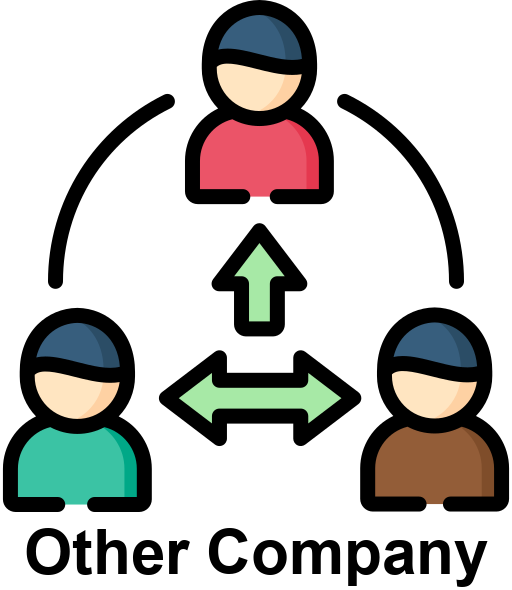
\includegraphics[width=12mm, valign=mc]{images/thirdparty_modified}
			
\includegraphics[width=12mm, valign=mc]{images/policeman_modified}
			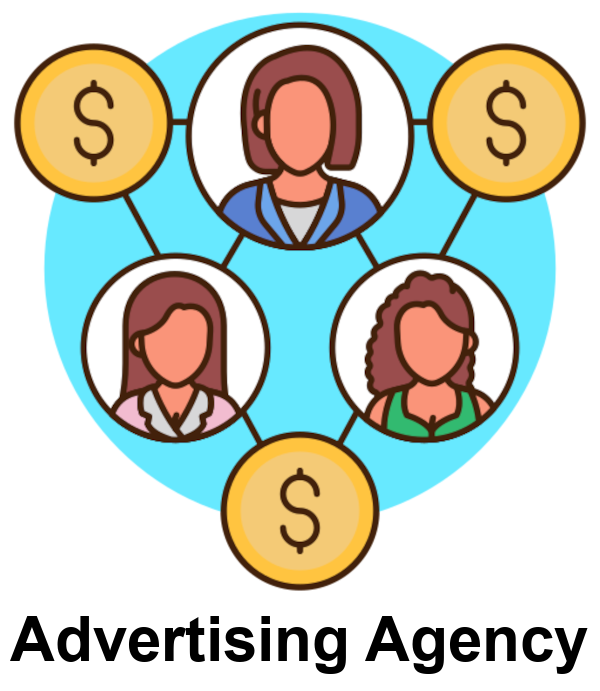
\includegraphics[width=12mm, valign=mc]{images/affiliate_modified}
			
\includegraphics[width=12mm, valign=mc]{images/payment_modified} } \\ [0.5ex]
		\cline{2-3} &
		\specialcell{We Sell \\ Data To} & \specialcell{\\[-8pt]
			
\includegraphics[width=12mm, valign=mc]{images/no-sale_modified} } \\ [0.5ex]
		\cline{2-3} &
		\specialcell{Retention \\ Period} & \specialcell{\\[-8pt]
			
\includegraphics[width=12mm, valign=mc]{images/unknown_modified} } \\ [0.5ex]
		\hline
		\multirow{4}{*}{\rotatebox[origin=rc]{90}{\textbf{Machine Learning}}} &
		Accuracy & \specialcell{\\[-8pt]
			
\includegraphics[width=12mm, valign=mc]{images/unknown_modified} } \\ [0.5ex]
		\cline{2-3} &
		\specialcell{Fairness \\ and Bias} & \specialcell{\\[-8pt]
			
\includegraphics[width=12mm, valign=mc]{images/unknown_modified} } \\ [0.5ex]
		\cline{2-3} &
		\specialcell{Potential \\ Risk} & \specialcell{\\[-8pt]
			
\includegraphics[width=12mm, valign=mc]{images/unknown_modified} } \\ [0.5ex]
		\hline
		\multicolumn{3}{|c|}{\specialcell{\\[-8pt]\textbf{Source:} All images were downloaded from Flaticon.com}} \\ [0.5ex]
		\hline

	\end{tabular}

\end{document}


%		\caption{Visual FactSheet for ChatGPT }
%		\label{fig:ChatGPT}
%	\end{figure}
%		\begin{figure}[!t!]
%		\centering
%		\scalebox{1}[0.90]{%pdflatex VFS.tex
%pdftoppm -png VFS.pdf output

\documentclass{standalone}

\usepackage{graphicx}
\usepackage[export]{adjustbox}
\usepackage{multirow, multicol}

%\newcommand{\specialcell}[2][b]{\begin{tabular}[#1]{@{}c@{}}#2\end{tabular}}

\begin{document}

	\begin{tabular}{|c|c|c|}
%		\hline
%		\multicolumn{3}{|c|}{\specialcell{\\[-8pt] Equifax is a credit bureau providing online access to credit score and report, \\ credit monitoring, alerts and identity theft protection.}} \\ [0.5ex]
		\hline
		\specialcell{\textbf{\large {Group}}} & \textbf{\large {Action}} & \textbf{\large {Activity}} \\ [0.5ex]
		\hline
		\multirow{2}{*}{\rotatebox[origin=rc]{90}{\textbf{General}}}
		& \specialcell{You Must \\ be} & \specialcell{\\[-8pt]
			
\includegraphics[width=12mm, valign=mc]{images/18_modified}
		}\\[0.5ex]
		\cline{2-3}
		& \specialcell{You Must \\ Provide} & \specialcell{\\[-8pt]
			
\includegraphics[width=12mm, valign=mc]{images/accurate_modified} }\\[0.5ex]
		\cline{2-3}
		\hline
		\multirow{4}{*}{\rotatebox[origin=rc]{90}{\textbf{User Data}}} &
		\specialcell{We Collect \\ Your Data} & \specialcell{\\[-8pt]
			
\includegraphics[width=12mm, valign=mc]{images/id_modified} \hspace{0.2cm}
			
\includegraphics[width=12mm, valign=mc]{images/personalinformation_modified} \hspace{0.2cm}
			
\includegraphics[width=12mm, valign=mc]{images/selfie_modified}
			
\includegraphics[width=12mm, valign=mc]{images/smartphone_modified}
			
\includegraphics[width=12mm, valign=mc]{images/httpcookie_modified}
			
\includegraphics[width=12mm, valign=mc]{images/location_modified} \\
			
\includegraphics[width=12mm, valign=mc]{images/payment_modified}
			
\includegraphics[width=12mm, valign=mc]{images/monitoring_modified}
			
\includegraphics[width=12mm, valign=mc]{images/shopping-cart_modified}} \\ [0.5ex]
		\cline{2-3} &
		\specialcell{We Process \\ Data For} & \specialcell{\\[-8pt]
			
\includegraphics[width=12mm, valign=mc]{images/gear_modified}
			
\includegraphics[width=12mm, valign=mc]{images/research_modified}
			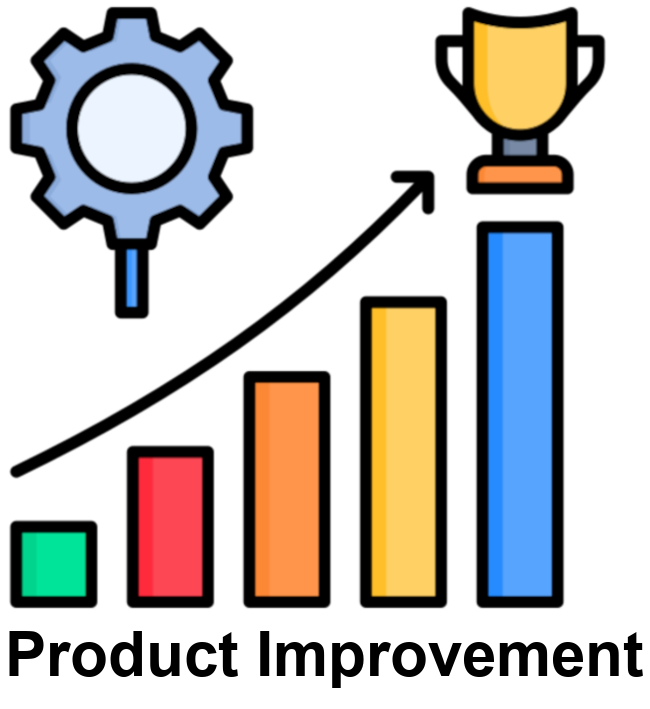
\includegraphics[width=12mm, valign=mc]{images/improvement_modified}
			
\includegraphics[width=12mm, valign=mc]{images/product-development_modified} } \\ [0.5ex]
		\cline{2-3} &
		\specialcell{We Share \\ Data With}  & \specialcell{\\[-8pt]
			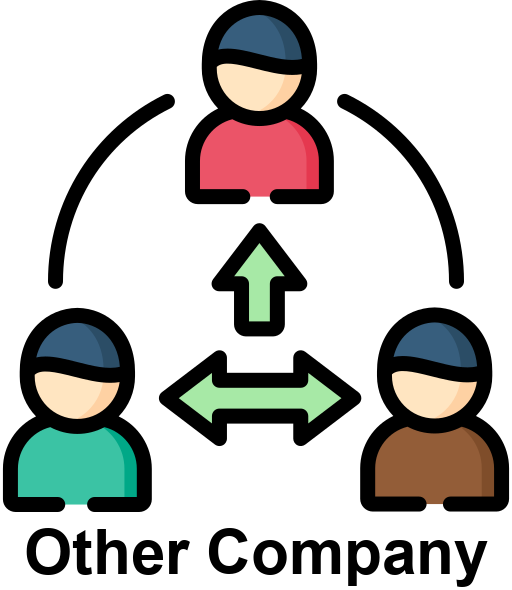
\includegraphics[width=12mm, valign=mc]{images/thirdparty_modified}
			
\includegraphics[width=12mm, valign=mc]{images/policeman_modified}
			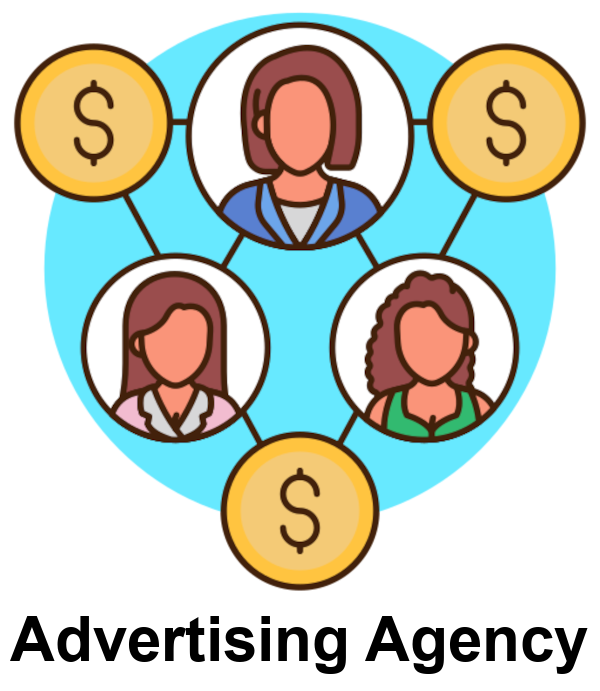
\includegraphics[width=12mm, valign=mc]{images/affiliate_modified}
			
\includegraphics[width=12mm, valign=mc]{images/payment_modified} } \\ [0.5ex]
		\cline{2-3} &
		\specialcell{We Sell \\ Data To} & \specialcell{\\[-8pt]
			
\includegraphics[width=12mm, valign=mc]{images/job_modified}
			
\includegraphics[width=12mm, valign=mc]{images/insurance-company_modified}
			
\includegraphics[width=12mm, valign=mc]{images/policeman_modified}} \\ [0.5ex]
		\cline{2-3} &
		\specialcell{Retention \\ Period} & \specialcell{\\[-8pt]
			
\includegraphics[width=12mm, valign=mc]{images/unknown_modified} } \\ [0.5ex]
		\hline
		\multirow{4}{*}{\rotatebox[origin=rc]{90}{\textbf{Machine Learning}}} &
		Accuracy & \specialcell{\\[-8pt]
			
\includegraphics[width=12mm, valign=mc]{images/unknown_modified} } \\ [0.5ex]
		\cline{2-3} &
		\specialcell{Fairness \\ and Bias} & \specialcell{\\[-8pt]
			
\includegraphics[width=12mm, valign=mc]{images/unknown_modified} } \\ [0.5ex]
		\cline{2-3} &
		\specialcell{Potential \\ Risk} & \specialcell{\\[-8pt]
			
\includegraphics[width=12mm, valign=mc]{images/unknown_modified} } \\ [0.5ex]
		\hline
		\multicolumn{3}{|c|}{\specialcell{\\[-8pt]\textbf{Source:} All images were downloaded from Flaticon.com}} \\ [0.5ex]
		\hline
	\end{tabular}

\end{document}

}
%		\caption{Visual FactSheet for Equifax }
%		\Description{Visual FactSheet for Equifax}
%		\label{fig:Equifax}
%	\end{figure}
%	[scale=0.7]
	Equifax, one of the largest consumer reporting agency, is a global leader in data, analytics, and technology solutions, primarily functioning as a credit reporting agency. The company gathers consumer information, analyzes it to produce credit scores and detailed reports, and sells these reports to third parties \cite{house_Representatives}. Our review presented in Appendix \ref{appendix:a} Figure \ref{fig:Equifax} revealed that Equifax’s data collection strategy is similar to that of ChatGPT, but significantly broader. For instance, Equifax collects government issued identification details such as passports, Social Security numbers, and taxpayer identification numbers. Beyond this, it also captures device information used to access its services and monitors online activities, including search history, purchasing behavior, and employment history \cite{equifax}. Surprisingly, Equifax process personal data without explicit consent from users and offer no option to \enquote{opt out} \cite{house_Representatives}. This practice is reflected in their \enquote{Privacy Statement} as well which states they do not respond to browser based \enquote{do not track} requests \cite{equifax}. We were also surprised to find no reference to the use of AI or machine learning in Equifax’s \enquote{Terms of Use} or \enquote{Privacy Statement}. Yet, the company openly acknowledges employing advanced ML models to uncover deep patterns and enhance predictiveness of its credit assessments \cite{equifaxAI}. As a result, we were unable to provide details about their ML architecture, its accuracy, potential risks, or issues related to fairness and bias in the training data.

\section{User Survey}

	Making decisions with little or no information often leaves individuals feeling powerless and frustrated. This lack of clarity can lead to trust issues, particularly when sharing personal data without full control over its use. To address this, our proposed VFS aims to present the \enquote{Terms and Conditions} of a fictitious social media platform in a visual format, enabling users to make informed choices about whether to engage with the platform. The user survey was designed as an online multiple choice questionnaire, following guidelines outlined by Arlene Fink \cite{alma991013701999705153}. To conduct the survey, we created a fictitious social media platform along with corresponding \enquote{Terms and Conditions}. Our fictitious agreement is very similar to ChatGPT but not as extensive as Equifax. Using our VFS framework, we developed an end user focused presentation (Figure \ref{fig:VFS_Survey}). An open invitation (Appendix \ref{appendix:c}) was extended to students from a research university and employees of a selected information technology company to participate voluntarily. The survey consisted of three sections. In the first section, participants reviewed the fictitious “Terms and Conditions” in the traditional text based format and answered questions (Appendix \ref{appendix:b}) to assess their understanding. They were then asked whether they would use the platform. In the second section, the same “Terms and Conditions” were presented using the VFS framework (Figure \ref{fig:VFS_Survey}), supplemented by visual descriptions (Figure \ref{fig:VSLegends} and \ref{fig:surveyLegendsML}). Participants were again asked about their willingness to use the platform. Finally, we gathered feedback on their observations and the effectiveness of the VFS framework. The survey findings are presented in Section \ref{surveyResult}.

	\begin{figure}[!t]
		\begin{minipage}{0.48\textwidth}
			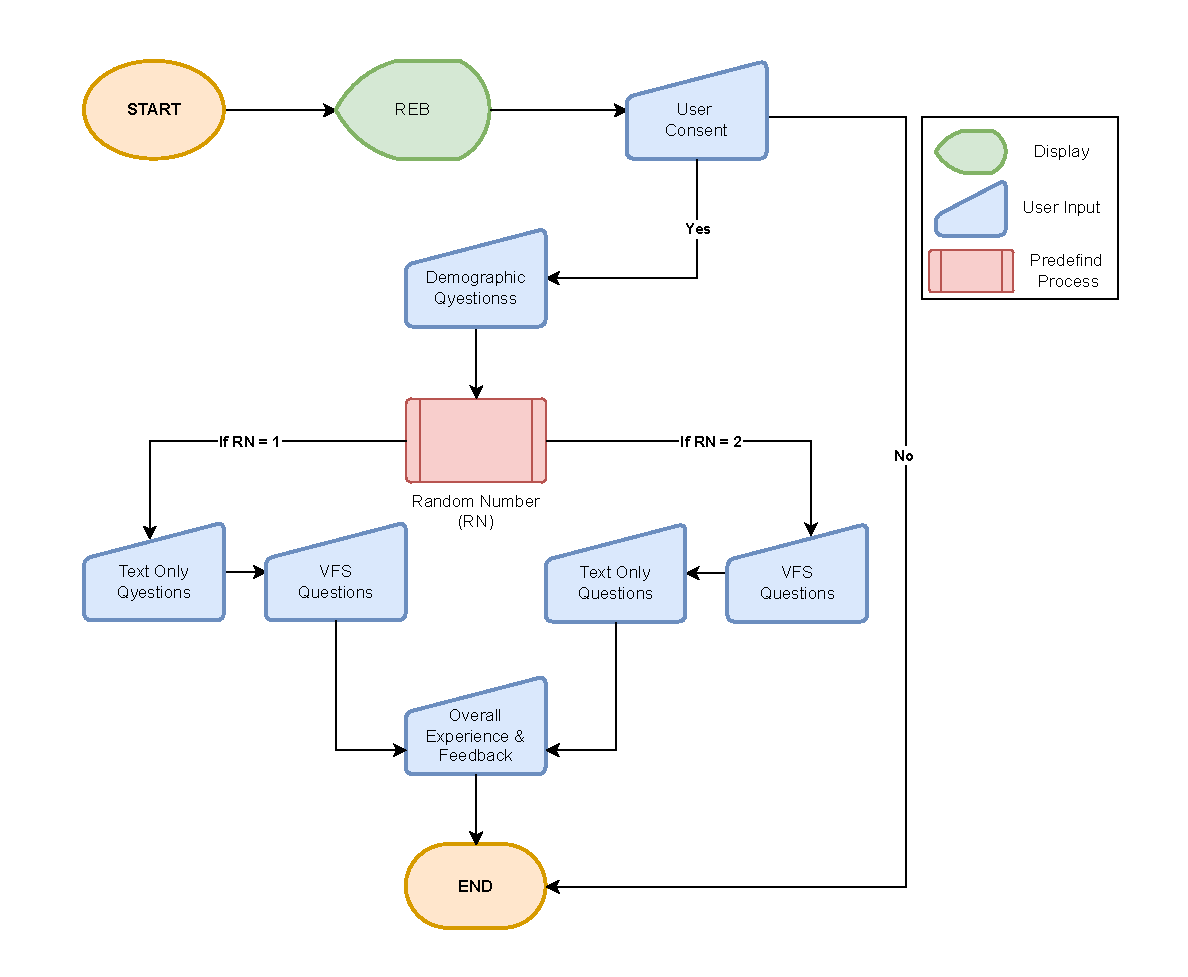
\includegraphics[page=1, scale=0.4]{images/pilotsurvey/SurveyQuestion_main.pdf}
			\caption{Survey Flow}
			\label{fig:SuveryFlow}
		\end{minipage}
		\hfill % Adds spacing between the two
		\begin{minipage}{0.48\textwidth}
			\scalebox{0.5}{%pdflatex VFS.tex
%pdftoppm -png VFS.pdf output

\documentclass{standalone}

\usepackage{graphicx}
\usepackage[export]{adjustbox}
\usepackage{multirow, multicol}
\usepackage{array}
%\newcommand{\specialcell}[2][b]{\begin{tabular}[#1]{@{}c@{}}#2\end{tabular}}
\graphicspath{{C:/MyFolder/Working_Papers/Working_Papers/facct_conf/}}
\newcolumntype{C}[1]{>{\centering\arraybackslash}p{#1}}

\begin{document}
	
	\begin{tabular}{|c|W{C}{8em}|c|}
	\hline
%	\multicolumn{3}{|c|}{\specialcell{\\[-8pt] \large {Social Media Platform Terms \& Conditions}}} \\ [0.5ex]
%	\hline
	\specialcell{\\[-8pt] \textbf{\large {Category}}} & \textbf{\large {Action}} & \textbf{\large {Activity}} \\ [0.5ex]
	\hline
	\multirow{2}{*}{\rotatebox[origin=rc]{360}{\textbf{General}}} 
	& \specialcell{You Must be} & \specialcell{\\[-8pt] 
		
\includegraphics[width=12mm, valign=mc]{images/16_modified} 
	}\\[0.5ex]
	\cline{2-3}
	& \specialcell{You Must Provide} & \specialcell{\\[-8pt]
		
\includegraphics[width=12mm, valign=mc]{images/accurate_modified} }\\[0.5ex]
	\cline{2-3}
	\hline
	\multirow{4}{*}{\rotatebox[origin=rc]{360}{\textbf{User Data}}}
	& \specialcell{We Collect} & \specialcell{\\[-8pt]
		
\includegraphics[width=12mm, valign=mc]{images/socialmedia_modified} \hspace{0.5mm}
		
\includegraphics[width=12mm, valign=mc]{images/personalinformation_modified} \hspace{0.5mm}
		
\includegraphics[width=12mm, valign=mc]{images/payment_modified} \hspace{0.5mm}
		
\includegraphics[width=12mm, valign=mc]{images/selfie_modified} \hspace{0.5mm}
		
\includegraphics[width=12mm, valign=mc]{images/location_modified} \hspace{0.5mm}
		
\includegraphics[width=12mm, valign=mc]{images/smartphone_modified} }\\[0.5ex]
	\cline{2-3}
	& \specialcell{We Process For} & \specialcell{\\[-8pt]
		
\includegraphics[width=12mm, valign=mc]{images/gear_modified} \hspace{0.5mm}
		
\includegraphics[width=12mm, valign=mc]{images/product-development_modified} } \\[0.5ex]
	\cline{2-3}
	& \specialcell{We Share With} & \specialcell{\\[-8pt]
		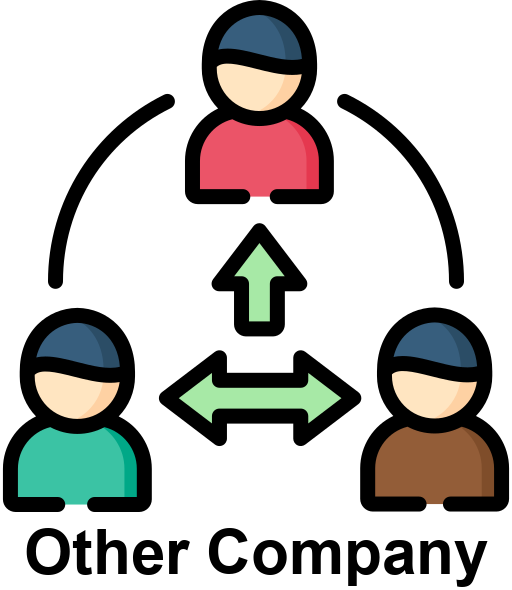
\includegraphics[width=12mm, valign=mc]{images/thirdparty_modified} \hspace{0.5mm}
		
\includegraphics[width=12mm, valign=mc]{images/policeman_modified}} \\[0.5ex]
	\cline{2-3}
	& \specialcell{We Sell To} & \specialcell{\\[-8pt]
		
\includegraphics[width=12mm, valign=mc]{images/job_modified} \hspace{0.5mm}
		
\includegraphics[width=12mm, valign=mc]{images/insurance-company_modified}} \\ [0.5ex]
	\cline{2-3}
	\hline
	\multirow{3}{*}{\rotatebox[origin=rc]{360}{\textbf{Machine Learning}}} 
	& \specialcell{Accuracy} & \specialcell{\\[-8pt] 
		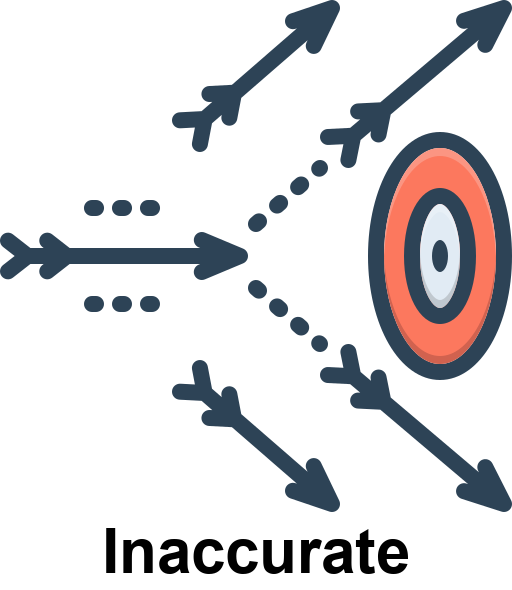
\includegraphics[width=12mm, valign=mc]{images/wrong_modified} } \\ [0.5ex]
	\cline{2-3}
	& Fairness & \specialcell{\\[-8pt] 
		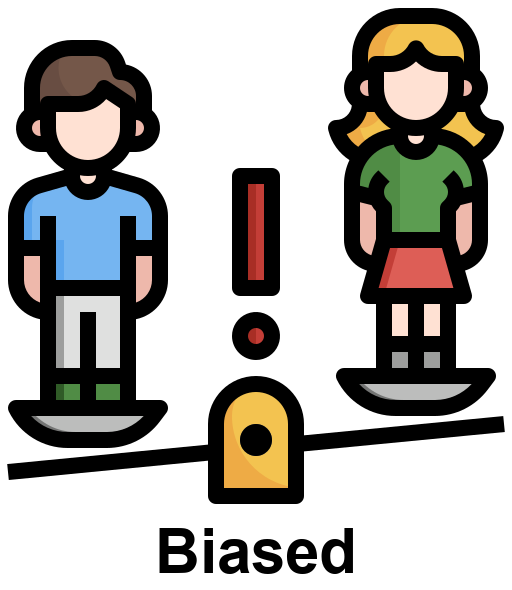
\includegraphics[width=12mm, valign=mc]{images/discrimination_modified} } \\ [0.5ex]
	\cline{2-3}
	& \specialcell{Potential Risk} & \specialcell{\\[-8pt] 
		
\includegraphics[width=12mm, valign=mc]{images/risk_modified} } \\ [0.5ex]
	\cline{2-3}
	\hline
	\multicolumn{3}{|c|}{\specialcell{\\[-8pt]\textbf{Source:} All images were downloaded from Flaticon.com}} \\ [0.5ex]
	\hline
	\end{tabular}

\end{document}

}
			\caption{Visual FactSheet for Social Media Platform}
			\label{fig:VFS_Survey}
		\end{minipage}
	\end{figure}

%	\begin{figure}[H]
%		\centering
%		\scalebox{0.85}[0.85] {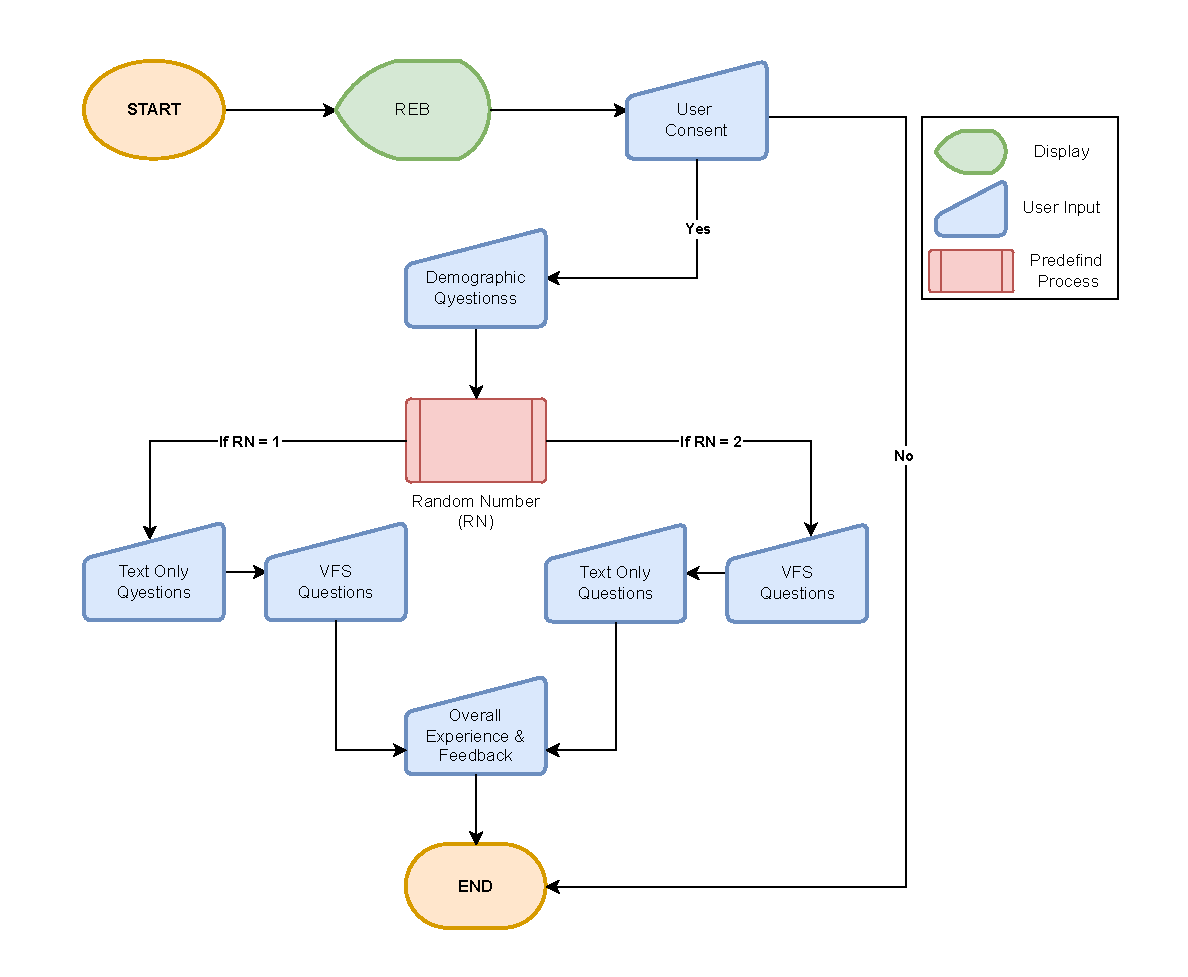
\includegraphics[page=1, width=\linewidth]{images/pilotsurvey/SurveyQuestion_main.pdf}}
%		\caption{Survey Flow}
%		\label{fig:SuveryFlow}
%	\end{figure}

%	\begin{figure}[h!]
%		\centering
%		\scalebox{1}[0.90]{%pdflatex VFS.tex
%pdftoppm -png VFS.pdf output

\documentclass{standalone}

\usepackage{graphicx}
\usepackage[export]{adjustbox}
\usepackage{multirow, multicol}
\usepackage{array}
%\newcommand{\specialcell}[2][b]{\begin{tabular}[#1]{@{}c@{}}#2\end{tabular}}
\graphicspath{{C:/MyFolder/Working_Papers/Working_Papers/facct_conf/}}
\newcolumntype{C}[1]{>{\centering\arraybackslash}p{#1}}

\begin{document}
	
	\begin{tabular}{|c|W{C}{8em}|c|}
	\hline
%	\multicolumn{3}{|c|}{\specialcell{\\[-8pt] \large {Social Media Platform Terms \& Conditions}}} \\ [0.5ex]
%	\hline
	\specialcell{\\[-8pt] \textbf{\large {Category}}} & \textbf{\large {Action}} & \textbf{\large {Activity}} \\ [0.5ex]
	\hline
	\multirow{2}{*}{\rotatebox[origin=rc]{360}{\textbf{General}}} 
	& \specialcell{You Must be} & \specialcell{\\[-8pt] 
		
\includegraphics[width=12mm, valign=mc]{images/16_modified} 
	}\\[0.5ex]
	\cline{2-3}
	& \specialcell{You Must Provide} & \specialcell{\\[-8pt]
		
\includegraphics[width=12mm, valign=mc]{images/accurate_modified} }\\[0.5ex]
	\cline{2-3}
	\hline
	\multirow{4}{*}{\rotatebox[origin=rc]{360}{\textbf{User Data}}}
	& \specialcell{We Collect} & \specialcell{\\[-8pt]
		
\includegraphics[width=12mm, valign=mc]{images/socialmedia_modified} \hspace{0.5mm}
		
\includegraphics[width=12mm, valign=mc]{images/personalinformation_modified} \hspace{0.5mm}
		
\includegraphics[width=12mm, valign=mc]{images/payment_modified} \hspace{0.5mm}
		
\includegraphics[width=12mm, valign=mc]{images/selfie_modified} \hspace{0.5mm}
		
\includegraphics[width=12mm, valign=mc]{images/location_modified} \hspace{0.5mm}
		
\includegraphics[width=12mm, valign=mc]{images/smartphone_modified} }\\[0.5ex]
	\cline{2-3}
	& \specialcell{We Process For} & \specialcell{\\[-8pt]
		
\includegraphics[width=12mm, valign=mc]{images/gear_modified} \hspace{0.5mm}
		
\includegraphics[width=12mm, valign=mc]{images/product-development_modified} } \\[0.5ex]
	\cline{2-3}
	& \specialcell{We Share With} & \specialcell{\\[-8pt]
		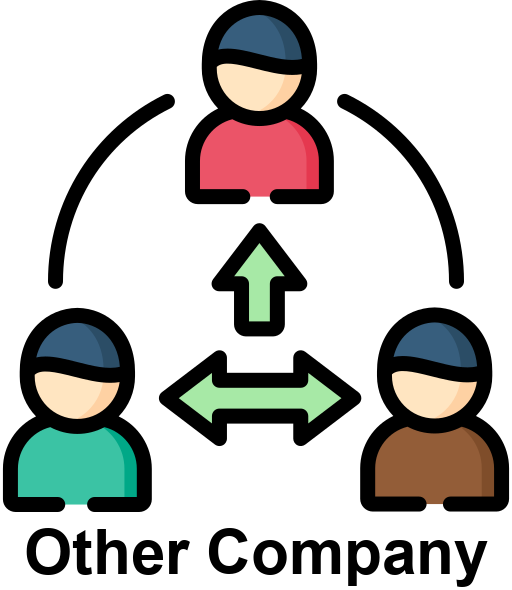
\includegraphics[width=12mm, valign=mc]{images/thirdparty_modified} \hspace{0.5mm}
		
\includegraphics[width=12mm, valign=mc]{images/policeman_modified}} \\[0.5ex]
	\cline{2-3}
	& \specialcell{We Sell To} & \specialcell{\\[-8pt]
		
\includegraphics[width=12mm, valign=mc]{images/job_modified} \hspace{0.5mm}
		
\includegraphics[width=12mm, valign=mc]{images/insurance-company_modified}} \\ [0.5ex]
	\cline{2-3}
	\hline
	\multirow{3}{*}{\rotatebox[origin=rc]{360}{\textbf{Machine Learning}}} 
	& \specialcell{Accuracy} & \specialcell{\\[-8pt] 
		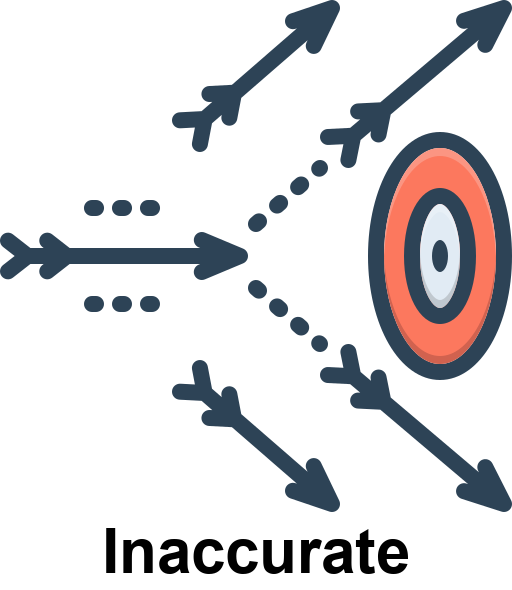
\includegraphics[width=12mm, valign=mc]{images/wrong_modified} } \\ [0.5ex]
	\cline{2-3}
	& Fairness & \specialcell{\\[-8pt] 
		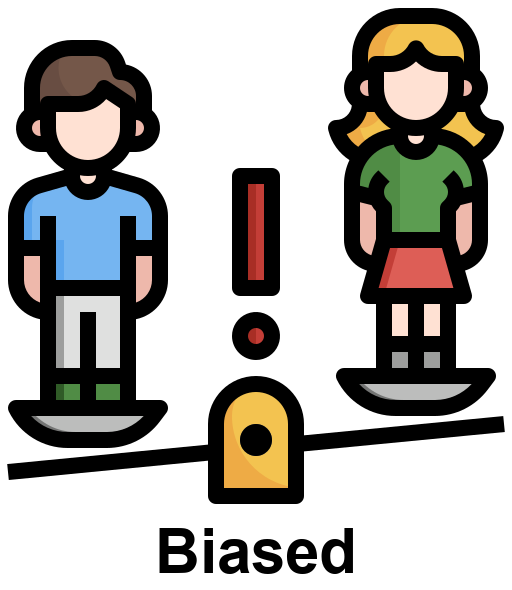
\includegraphics[width=12mm, valign=mc]{images/discrimination_modified} } \\ [0.5ex]
	\cline{2-3}
	& \specialcell{Potential Risk} & \specialcell{\\[-8pt] 
		
\includegraphics[width=12mm, valign=mc]{images/risk_modified} } \\ [0.5ex]
	\cline{2-3}
	\hline
	\multicolumn{3}{|c|}{\specialcell{\\[-8pt]\textbf{Source:} All images were downloaded from Flaticon.com}} \\ [0.5ex]
	\hline
	\end{tabular}

\end{document}

}
%		\caption{Visual FactSheet for Social Media Platform}
%		\label{fig:VFS_Survey}
%	\end{figure}

\subsection{Survey Design}

	The survey consists of seven sections. The first section, Informed Consent, provides participants with essential information about the purpose and context of the study.

	\begin{enumerate}
		\item Demography
		\item Data Collection
		\item Data Processing
		\item Data Retention
		\item Data Share
		\item Accuracy, Fairness, and Bias
		\item Potential Risk
	\end{enumerate}

	\subsubsection{Demography }
	A VFS must start with the purpose of the AIS service. This should provide an example problem and how the AIS service is solving it.

	\begin{figure}[!t]
		\begin{minipage}{0.48\textwidth}
			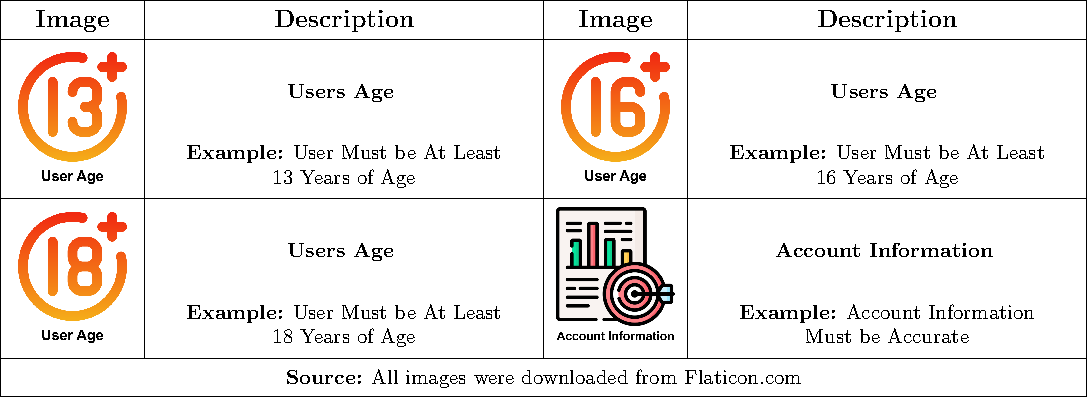
\includegraphics[page=1, scale=0.4]{diagram/Survey_Legends_01.pdf}
			\caption{Survey Legends (Demography)}
			\label{fig:Survey_Legends_01}
		\end{minipage}
		\hfill % Adds spacing between the two
		\begin{minipage}{0.48\textwidth}
			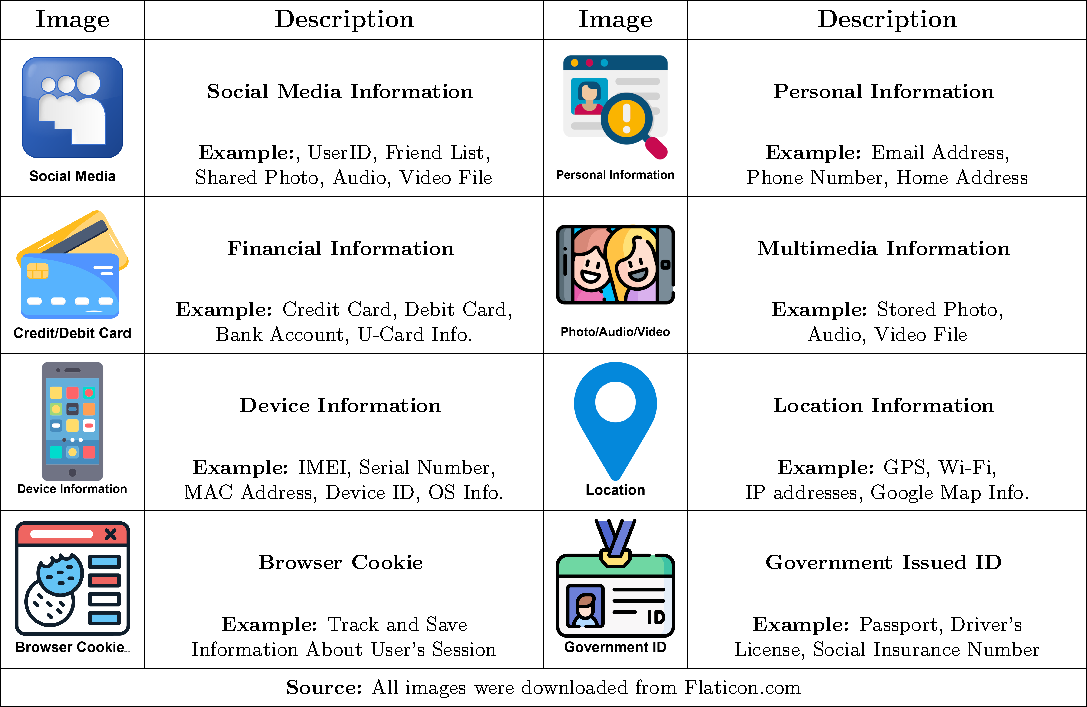
\includegraphics[page=1, scale=0.4]{diagram/Survey_Legends_02.pdf}
			\caption{Survey Legends (Data Collection)}
			\label{fig:Survey_Legends_02}
		\end{minipage}
	\end{figure}

%	\begin{figure}[!h]
%		\centering
%		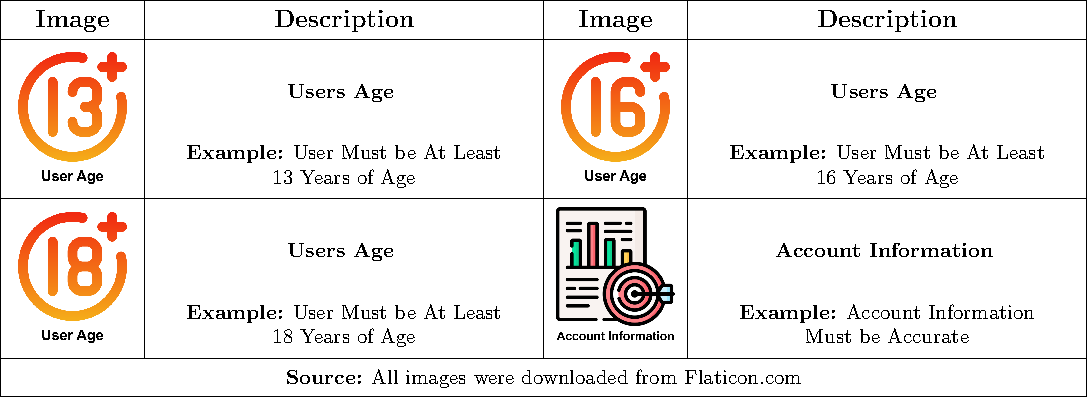
\includegraphics[page=1, width=\linewidth]{diagram/Survey_Legends_01.pdf}
%		\caption{Survey Legends (Demography)}
%		\label{fig:Survey_Legends_01}
%	\end{figure}

	\subsubsection{Data Collection }
	An AIS user must know what type of data the AIS provider will be collecting (if any) while using it. The AIS provider may or may not provide an example informing the user what type of data will be collected. It is highly recommended that the AIS provider will provide an example. The minimum requirement of this step can be an acknowledgment from the AIS provider in the form of a \enquote{Yes} or \enquote{No}.

%	\begin{figure}[!h]
%		\centering
%		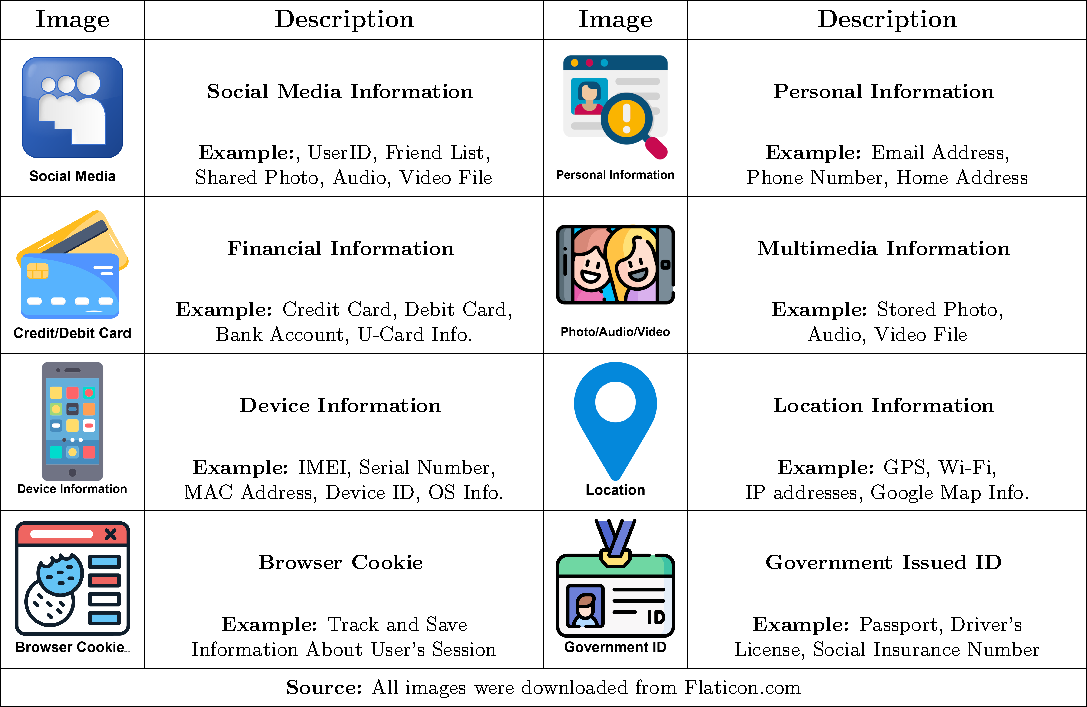
\includegraphics[page=1, width=\linewidth]{diagram/Survey_Legends_02.pdf}
%		\caption{Survey Legends (Data Collection)}
%		\label{fig:Survey_Legends_02}
%	\end{figure}

	\subsubsection{Data Processing }
	If the AIS provider acknowledges that they collect user data, the provider must inform users why they collect it and how user data will be processed for future use. The provider must also inform users how they make sure collected data is free from PII. The minimum requirement of this step can be an acknowledgment from the AIS provider as a form of a \enquote{Yes} or \enquote{No}.

	\begin{figure}[!t]
		\begin{minipage}{0.48\textwidth}
			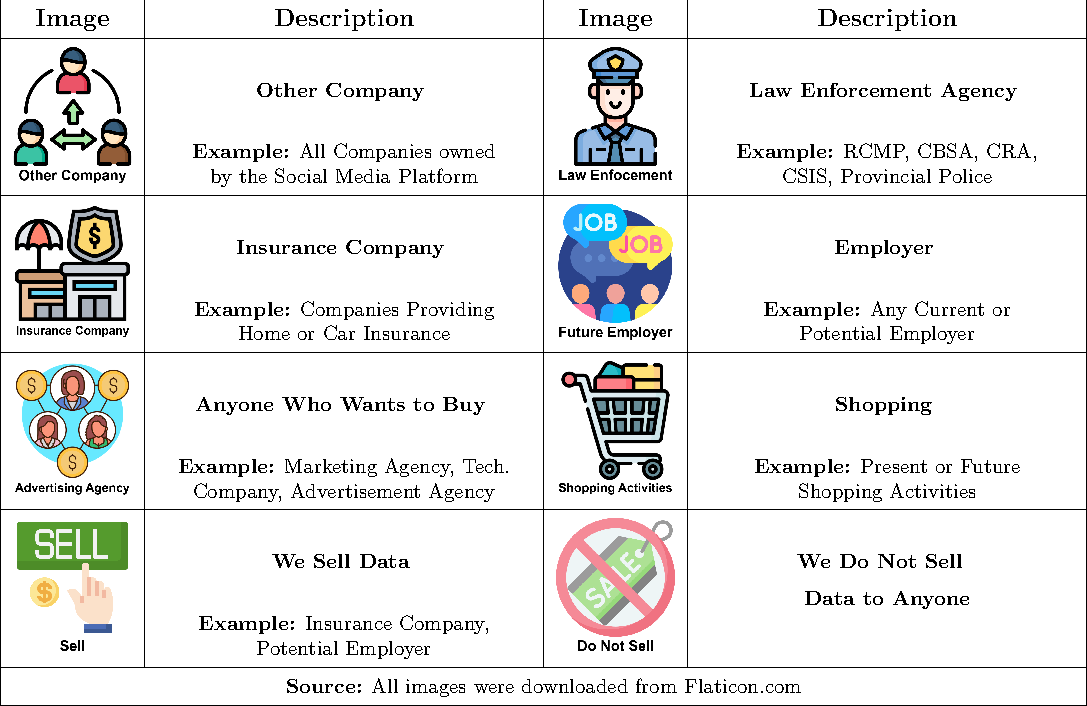
\includegraphics[page=1, scale=0.4]{diagram/Survey_Legends_03.pdf}
			\caption{Survey Legends (Data Processing)}
			\label{fig:Survey_Legends_03}
		\end{minipage}
		\hfill % Adds spacing between the two
		\begin{minipage}{0.48\textwidth}
			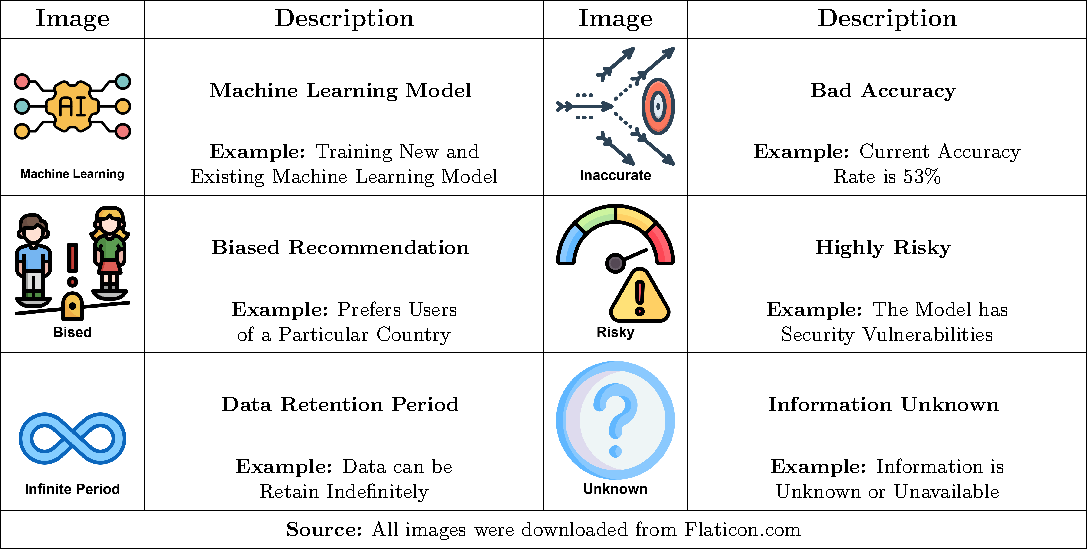
\includegraphics[page=1, scale=0.4]{diagram/Survey_Legends_04.pdf}
			\caption{Survey Legends (Machine Learning)}
			\label{fig:Survey_Legends_04}
		\end{minipage}
	\end{figure}

%	\begin{figure}[!h]
%		\centering
%		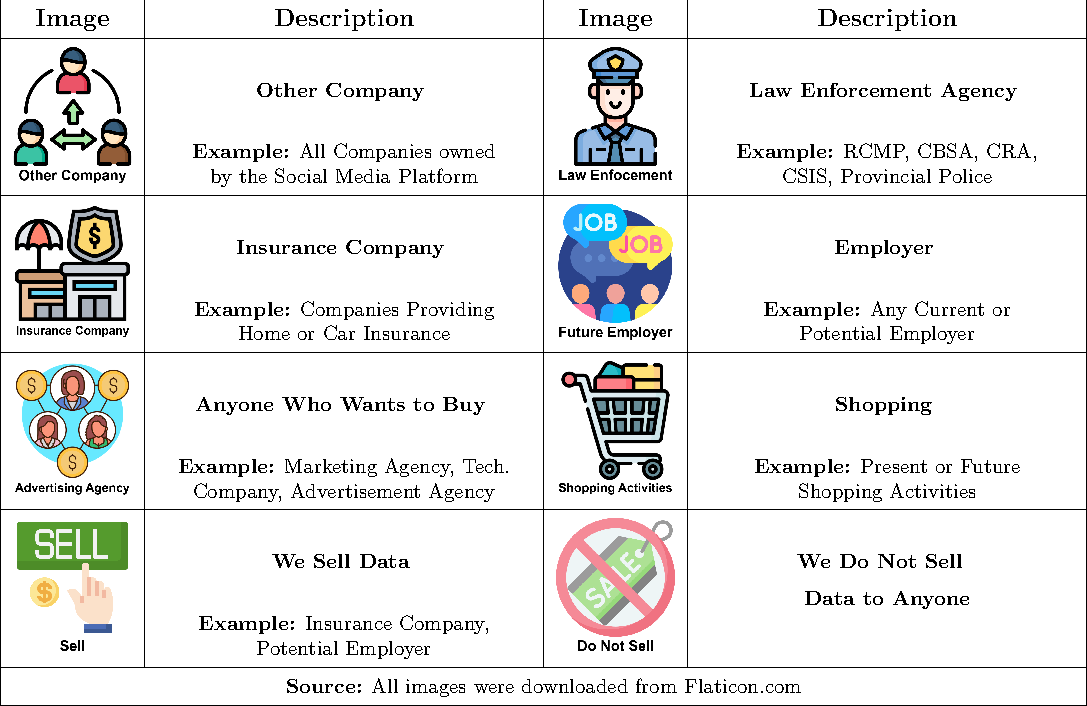
\includegraphics[page=1, width=\linewidth]{diagram/Survey_Legends_03.pdf}
%		\caption{Survey Legends (Data Processing)}
%		\label{fig:Survey_Legends_03}
%	\end{figure}

	\subsubsection{Data Retention }
	If the AIS provider collects and processes user data, the provider must inform users of their data retention policy. They must also inform users how they destroy user data once the retention period is over.

	\subsubsection{Data Share}
	AIS providers often share collected data with their affiliates, government organizations, e.g., law enforcement agencies, and third party AIS providers. They also share and transfer ownership of collected data in the occurrence of business transfer. It is necessary for the provider to inform users with whom they intend to share collected data and in what form, i.e., unprocessed or processed.

	\subsubsection{Accuracy, Fairness, and Bias }
	Regardless of free or paid services, it is mandatory for the AIS provider to show evidence about the effectiveness and usefulness of the service they are offering. For AIS underlying ML models' accuracy is a widely accepted metric for such \cite{blagec_critical_2020}. Since there is a concern about unfair and biased recommendations or decisions, it is the provider's responsibility to inform its users of the level of fair and unbiased recommendations or decisions of their service. The minimum requirement of this step can be a percentile of accuracy, fairness, and biasness.

%	\begin{figure}[!h]
%		\centering
%		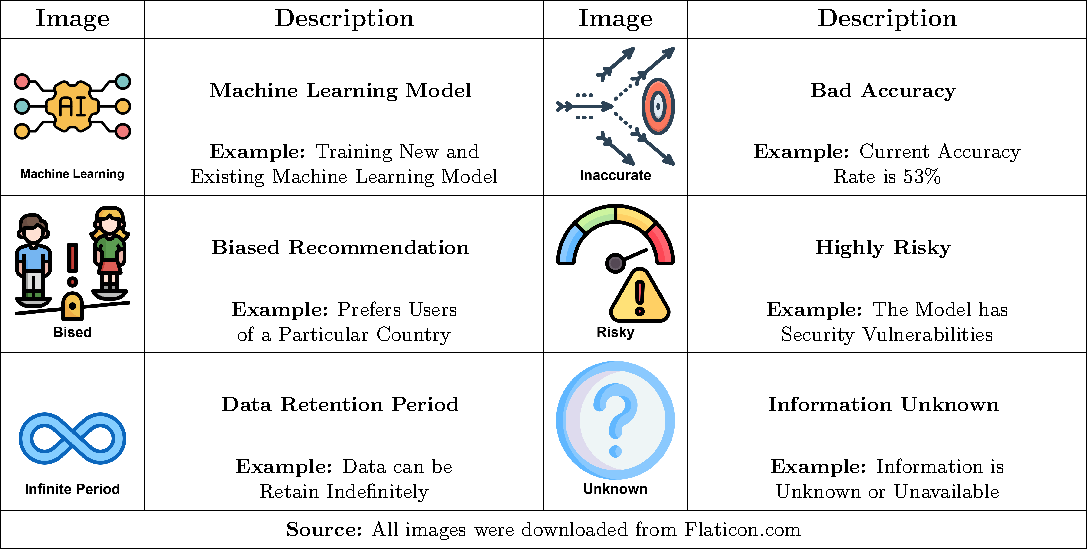
\includegraphics[page=1, width=\linewidth]{diagram/Survey_Legends_04.pdf}
%		\caption{Survey Legends (Machine Learning)}
%		\label{fig:Survey_Legends_04}
%	\end{figure}

	\subsubsection{Potential Risk }
	AISs are not free from potential risk. There is a growing concern about adversarial attacks on the underlying ML models along with training data poisoning, stealing, and model hijacking. The AIS provider must acknowledge if there is any potential risk for using the service and how the provider minimizes or eliminates those potential risks.

	The demographic section of the survey collects information about participants’ educational background, gender, and age. These data are essential for analyzing the survey results. In the following section, participants are presented with a short story introducing a new social media website. They are then instructed to review two different versions of the platform’s terms and conditions and respond to related questions

	Figure \ref{fig:VFS} presented below shows the equivalent VFS of the hypothetical social media platform.

%	\begin{figure}[!h]
%		\centering
%		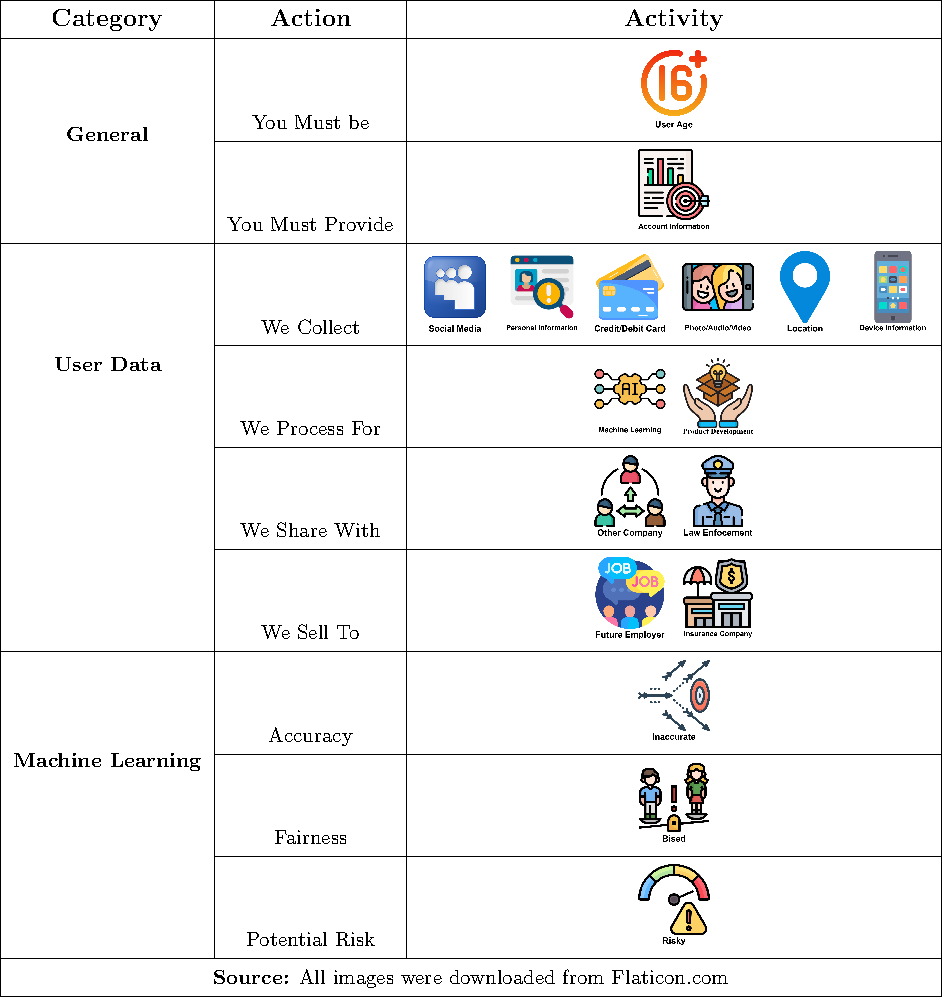
\includegraphics[page=1, width=\linewidth]{diagram/Survey_VFS.pdf}
%		\caption{VFS}
%		\label{fig:VFS}
%	\end{figure}


\section{Participant Sampling and Technology}
	As mentioned earlier, each participant was presented with two versions of the T\&C: a traditional text‑only T\&C and its corresponding Visual T\&C. A random number between 1 and 2 was generated within the Qualtrics platform to determine the presentation order. This ensured that participants viewed either the text‑only T\&C first or the Visual T\&C first. Figure \ref{fig:SuveryFlow} illustrates the complete survey flow, which consists of seven sections in which participants provide their responses.

	Because the social media scenario used in this study is entirely fictional, a hypothetical T\&C was developed for the project and is provided in Appendix XXX. This T\&C was created using Microsoft Co-Pilot and is modeled after the structure commonly found in commercial social media platforms such as Facebook. To produce a corresponding Visual T\&C, the project adopted the framework outlined in Section \ref{ComponentsVFS}. Figure \ref{fig:Survey_Legends_02} shows a subset of the images used to construct the Visual FactSheet (VFS) equivalent.

\section{Pilot Result}\label{pilotsurvey}

	Following ethics approval, the survey was implemented using Qualtrics and piloted with a small cohort of graduate students and faculty members from the UNB Department of Computer Science. The pilot results are presented in the following sub sections.

\subsection{Demography}

	During the week long pilot run of the survey, 10 participants took part. Among them six completely, two partially, and two did not complete the survey. However, even with this small number of participants, it was observed that the are demographically diverse. Figure \ref{fig:gender} shows how participants identifies themselves and highest education level achieved which spread in three levels.

	\begin{figure}[!h]
		\centering
		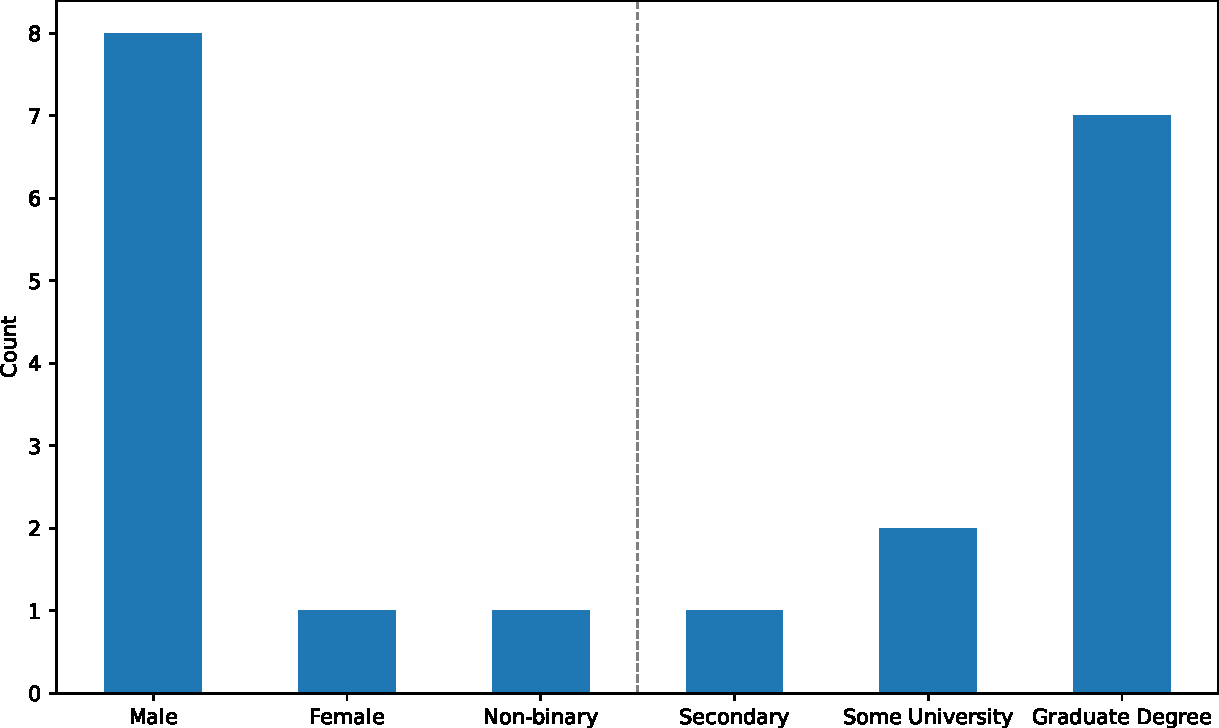
\includegraphics[ width=\linewidth]{images/pilotsurvey/Demography.pdf}
		\caption{Demography (Gender)}
		\label{fig:gender}
	\end{figure}

\subsection{Level of Understanding}

	The survey inquires participants level of understanding after reviewing text only and visual T\&C. Data collected through pilot survey shows that participants exhibit higher confidence level after reviewing visual T\&C. Figure \ref{fig:confidence} shows that mean confidence for visual T\&C is higher than that of text only T\&C.

	\begin{figure}[!h]
		\centering
		\scalebox{0.75}[0.75] {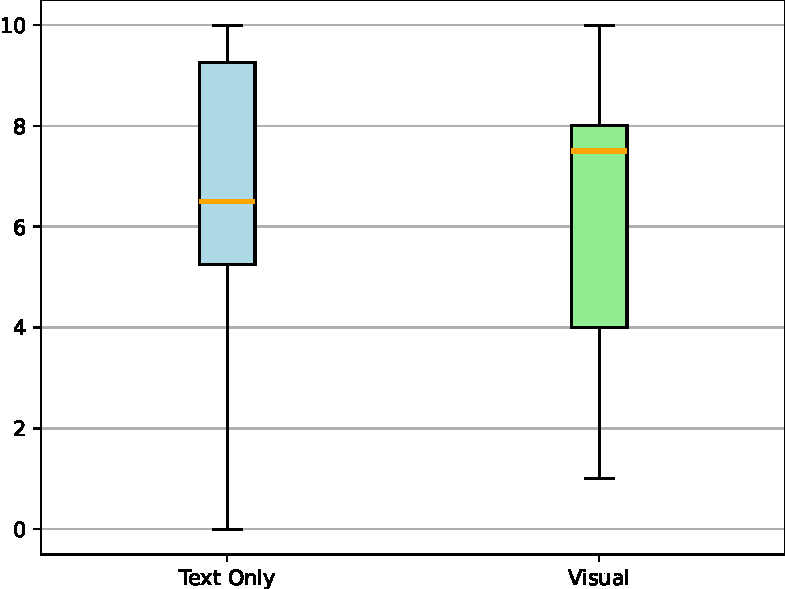
\includegraphics[page=1, width=\linewidth]{images/pilotsurvey/Survey_Pilot.pdf}}
		%		\includegraphics[ width=\linewidth]{images/Understanding_RatingT\&C.pdf}
		\caption{Confidence Understanding T\&C Agreement}
		\label{fig:confidence}
	\end{figure}

\subsection{NASA Task Load Index}

	The survey measured subjective workload after completing text only and visual T\&C following NASA TLX. Pilot survey data shows that participants experienced higher mental demand, shown in Figure \ref{fig:frustation} Question 1, interpreting text only T\&C. The mental demand was doubled in comparison to visual T\&C. Participants also exhibited higher frustration reading the text only T\&C. The frustration level again more than double than that of visual T\&C. Figure \ref{fig:frustation} Question 6, represents the data collected during pilot survey.

	\begin{figure}[!h]
		\centering
		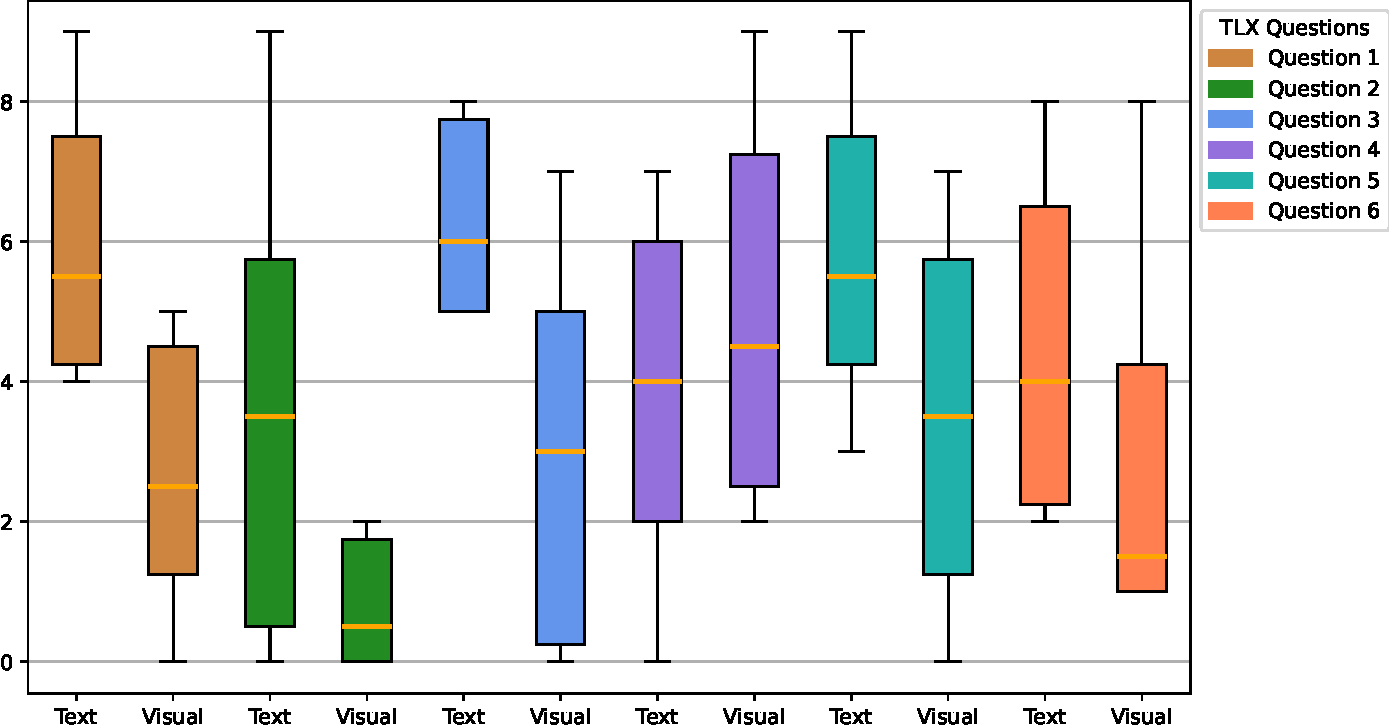
\includegraphics[width=\linewidth]{images/pilotsurvey/TLX.pdf}
		\caption{Frustration Reading T\&C}
		\label{fig:frustation}
	\end{figure}

\subsection{Time Vs Accuracy}

	During the pilot survey, it was discovered, presented in Figure \ref{fig:time} that almost all participants except one spent very less time reviewing text only and visual T\&C. However, participants were able to achieve higher accuracy answering survey questions that are directly related to the T\&C. For example, when asked about information sharing with their potential employer, participants were able to answer more accurately after reviewing visual T\&C. Figure \ref{fig:employer} shows that less participants were unsure and more participants were aware of this fact.

	\begin{figure}[!h]
		\centering
		\scalebox{0.75}[0.75] {\includegraphics[page=8, width=\linewidth]{images/pilotsurvey/Survey_Pilot.pdf}}
		\caption{Time Spent Reviewing T\&C}
		\label{fig:time}
	\end{figure}

	\begin{figure}[!h]
		\centering
		\scalebox{0.75}[0.75] {\includegraphics[page=7, width=\linewidth]{images/pilotsurvey/Survey_Pilot.pdf}}
		\caption{Information Share with Employer}
		\label{fig:employer}
	\end{figure}

\subsection{T\&C Preference}

	At the end of the survey, participants were asked about T\&C preference, i.e., text only or visual. Data, presented in Figure \ref{fig:rating} shows that majority of participants chose visual over text only T\&C.

	\begin{figure}[!h]
		\centering
		\scalebox{0.75}[0.75] {\includegraphics[page=4, width=\linewidth]{images/pilotsurvey/Survey_Pilot.pdf}}
		\caption{T\&C Rating}
		\label{fig:rating}
	\end{figure}


\section{Live Survey}

	After the successful pilot phase, the full survey was launched for all intended participants. To promote participation, the survey was distributed as a news article through the UNB faculty, staff, and student news portal (see Appendix XXX). The survey remains active, although it has not yet been circulated other media channels except UNB.

\subsection{Result}


%https://www.heinz.cmu.edu/~acquisti/papers/Acquisti_Toggles_DollarSigns_Triangles_Convey_Privacy_Icons_LinkTexts.pdf
\section{Conclusion and Limitation}

	In this paper, we defined four types of FS by identifying and categorizing distinct user groups and introduce a methodology for developing a VFS for ML services. Our proposed FS definitions aim to reduce ambiguity for FS creators and generators. We further believe that the VFS will empower an increasing number of ML service consumers by safeguarding their rights and enabling informed decisions when using publicly available free ML services. Although we present four FS types with corresponding definitions, our primary focus is on the end-user category. All icons used in the VFS design are generic, publicly available, and sourced from Flaticon.com. We see potential for standardizing these icons and plan to conduct a survey experiment to evaluate the strengths and weaknesses of the proposed VFS, continuing our efforts toward icon standardization.


\section{Acknowledgments}

%%
%% The next two lines define the bibliography style to be used, and
%% the bibliography file.
\bibliographystyle{ACM-Reference-Format}
\bibliography{hci}

%%
%% If your work has an appendix, this is the place to put it.
\appendix

\section{Equifax} \label{appendix:a}

%	\begin{figure}[!t!]
%		\centering
%		\scalebox{1}[0.90]{%pdflatex VFS.tex
%pdftoppm -png VFS.pdf output

\documentclass{standalone}

\usepackage{graphicx}
\usepackage[export]{adjustbox}
\usepackage{multirow, multicol}

%\newcommand{\specialcell}[2][b]{\begin{tabular}[#1]{@{}c@{}}#2\end{tabular}}

\begin{document}

	\begin{tabular}{|c|c|c|}
%		\hline
%		\multicolumn{3}{|c|}{\specialcell{\\[-8pt] Equifax is a credit bureau providing online access to credit score and report, \\ credit monitoring, alerts and identity theft protection.}} \\ [0.5ex]
		\hline
		\specialcell{\textbf{\large {Group}}} & \textbf{\large {Action}} & \textbf{\large {Activity}} \\ [0.5ex]
		\hline
		\multirow{2}{*}{\rotatebox[origin=rc]{90}{\textbf{General}}}
		& \specialcell{You Must \\ be} & \specialcell{\\[-8pt]
			
\includegraphics[width=12mm, valign=mc]{images/18_modified}
		}\\[0.5ex]
		\cline{2-3}
		& \specialcell{You Must \\ Provide} & \specialcell{\\[-8pt]
			
\includegraphics[width=12mm, valign=mc]{images/accurate_modified} }\\[0.5ex]
		\cline{2-3}
		\hline
		\multirow{4}{*}{\rotatebox[origin=rc]{90}{\textbf{User Data}}} &
		\specialcell{We Collect \\ Your Data} & \specialcell{\\[-8pt]
			
\includegraphics[width=12mm, valign=mc]{images/id_modified} \hspace{0.2cm}
			
\includegraphics[width=12mm, valign=mc]{images/personalinformation_modified} \hspace{0.2cm}
			
\includegraphics[width=12mm, valign=mc]{images/selfie_modified}
			
\includegraphics[width=12mm, valign=mc]{images/smartphone_modified}
			
\includegraphics[width=12mm, valign=mc]{images/httpcookie_modified}
			
\includegraphics[width=12mm, valign=mc]{images/location_modified} \\
			
\includegraphics[width=12mm, valign=mc]{images/payment_modified}
			
\includegraphics[width=12mm, valign=mc]{images/monitoring_modified}
			
\includegraphics[width=12mm, valign=mc]{images/shopping-cart_modified}} \\ [0.5ex]
		\cline{2-3} &
		\specialcell{We Process \\ Data For} & \specialcell{\\[-8pt]
			
\includegraphics[width=12mm, valign=mc]{images/gear_modified}
			
\includegraphics[width=12mm, valign=mc]{images/research_modified}
			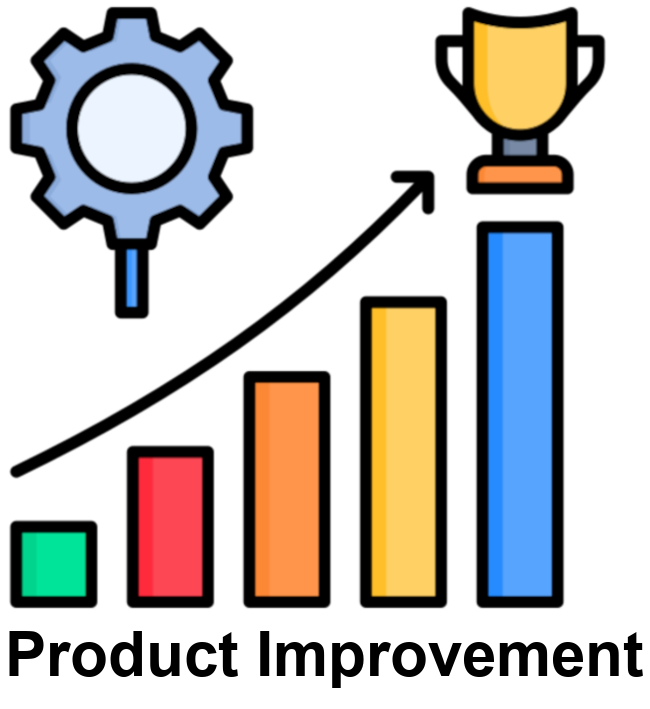
\includegraphics[width=12mm, valign=mc]{images/improvement_modified}
			
\includegraphics[width=12mm, valign=mc]{images/product-development_modified} } \\ [0.5ex]
		\cline{2-3} &
		\specialcell{We Share \\ Data With}  & \specialcell{\\[-8pt]
			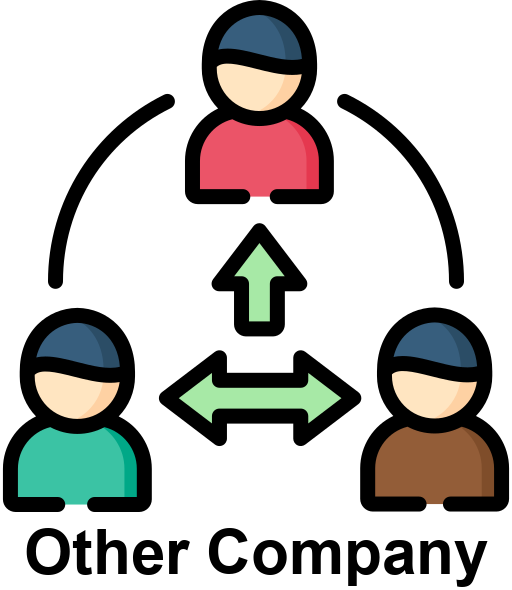
\includegraphics[width=12mm, valign=mc]{images/thirdparty_modified}
			
\includegraphics[width=12mm, valign=mc]{images/policeman_modified}
			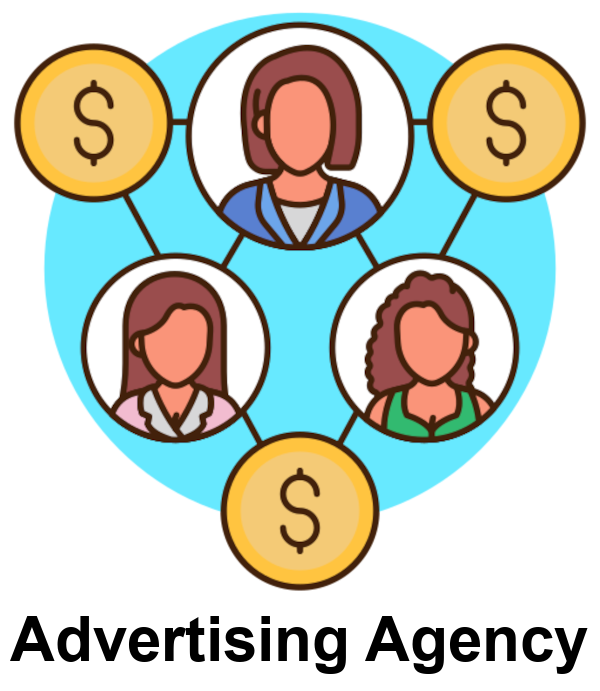
\includegraphics[width=12mm, valign=mc]{images/affiliate_modified}
			
\includegraphics[width=12mm, valign=mc]{images/payment_modified} } \\ [0.5ex]
		\cline{2-3} &
		\specialcell{We Sell \\ Data To} & \specialcell{\\[-8pt]
			
\includegraphics[width=12mm, valign=mc]{images/job_modified}
			
\includegraphics[width=12mm, valign=mc]{images/insurance-company_modified}
			
\includegraphics[width=12mm, valign=mc]{images/policeman_modified}} \\ [0.5ex]
		\cline{2-3} &
		\specialcell{Retention \\ Period} & \specialcell{\\[-8pt]
			
\includegraphics[width=12mm, valign=mc]{images/unknown_modified} } \\ [0.5ex]
		\hline
		\multirow{4}{*}{\rotatebox[origin=rc]{90}{\textbf{Machine Learning}}} &
		Accuracy & \specialcell{\\[-8pt]
			
\includegraphics[width=12mm, valign=mc]{images/unknown_modified} } \\ [0.5ex]
		\cline{2-3} &
		\specialcell{Fairness \\ and Bias} & \specialcell{\\[-8pt]
			
\includegraphics[width=12mm, valign=mc]{images/unknown_modified} } \\ [0.5ex]
		\cline{2-3} &
		\specialcell{Potential \\ Risk} & \specialcell{\\[-8pt]
			
\includegraphics[width=12mm, valign=mc]{images/unknown_modified} } \\ [0.5ex]
		\hline
		\multicolumn{3}{|c|}{\specialcell{\\[-8pt]\textbf{Source:} All images were downloaded from Flaticon.com}} \\ [0.5ex]
		\hline
	\end{tabular}

\end{document}

}
%		\caption{Visual FactSheet for Equifax }
%		\Description{Visual FactSheet for Equifax}
%		\label{fig:Equifax}
%	\end{figure}

	\section{Survey Story}

	\begin{lstlisting}[frame=single,upquote=false,breaklines=true,columns=fullflexible,columns=fullflexible,columns=fullflexible,breakindent=0pt,basicstyle=\ttfamily\small,captionpos=b,caption=Social Media Story,label=lst:story]
		Discover a Social Space Designed for You
		Most social media platforms today feel crowded, noisy, and designed to keep you scrolling rather than genuinely connecting. That is why we created something different, a platform that puts you at the center. Your interests, your comfort, and your voice shape your experience, not a one size fits all algorithms.

		Introducing Gaia, our new social media platform. Inspired by the Greek goddess who nurtures and sustains the world, Gaia is designed to be a space where meaningful connections can flourish. Our platform encourages responsible sharing and fosters a community built on positivity, mutual respect, and a sense of shared harmony.

		Here, advanced Machine Learning works quietly in the background to support you and not to manipulate you. Instead of pushing random content, our Machine Learning models help surface communities, conversations, and people who genuinely share your passions. The goal is not to keep you online longer; it is to help you find what matters faster.

		You will experience a calmer, more personal environment where your privacy is respected and your time is valued. Our Machine Learning assisted platform is designed with user controlled preferences, allowing you to customize what the platform learns, forgets, or ignores entirely. You are always in control.

		Gaia is not just another social media platform. It is a space built to help you connect, grow, and belong supported by intelligent tools that enhance real human connection rather than overshadow it.
	\end{lstlisting}
	\section{Survey Poster}
	\begin{figure}[!t]
		\centering
		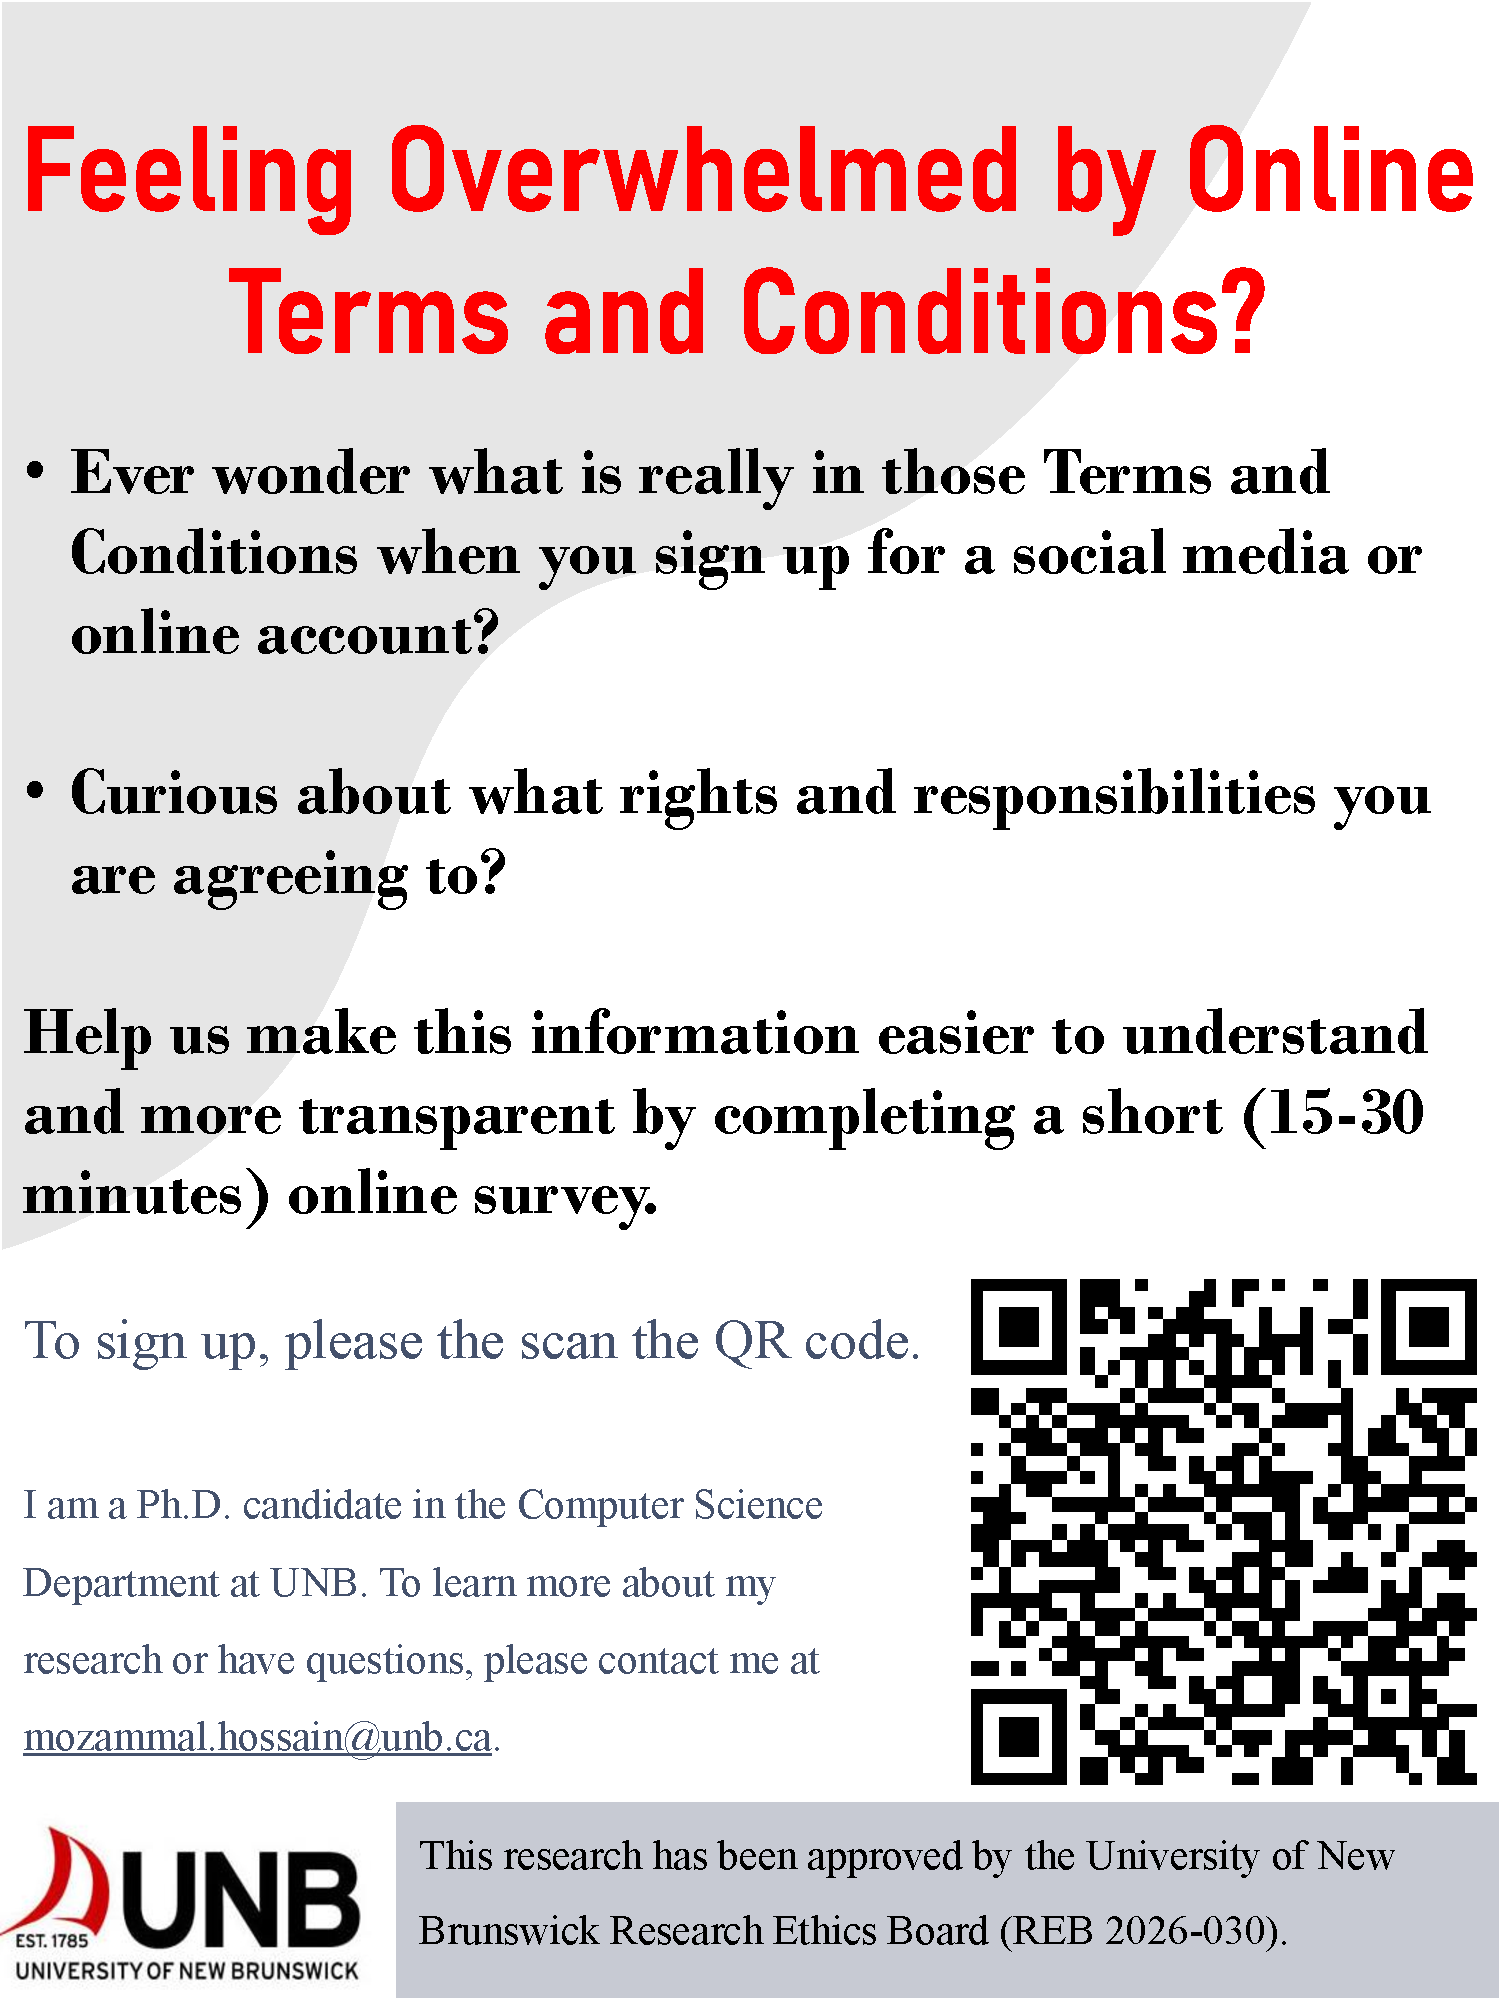
\includegraphics[scale=0.5]{diagram/Poster.pdf}
		\caption{Survey Poster}
		\label{fig:SuveryPoster}
	\end{figure}

\section{News Article}
\begin{lstlisting}[frame=single,upquote=false,breaklines=true,columns=fullflexible,columns=fullflexible,columns=fullflexible,breakindent=0pt,basicstyle=\ttfamily\small,captionpos=b,caption=Social Media Story,label=lst:news_article]

Article Title: Ever been overwhelmed by online Terms and Conditions? Complete an Online Survey to help us Design a Better Solution.

Article Details:
Ever wonder what is really in those Terms and Conditions when you sign up for a social media or online account? Curious about what rights and responsibilities you are agreeing to? Help us make this information easier to understand and more transparent by completing a short online research study.

1. The purpose of this study is to understand whether different ways of presenting Terms and Conditions agreements can affect,
2. How you read, interpret, and understand the underlying Term and Conditions that you are being asked to agree to, and

Your understanding of how your online data will be used including Machine Learning model development and improvement.

As a participant in this research study, you will review two different versions of a Terms and Conditions agreement for a fictitious Social Media Platform and complete a short survey that should take about 15-30 minutes.

My name is Mozammal Hossain. I am a PhD. candidate in the Computer Science Department at UNB.  I am conducting a short academic survey to explore this very topic, and your input would be incredibly valuable for my research. Participation involves completing a short online survey (15 to 30 minutes) and will help promote clear and fair software use for everyone.

To participate, please click here (https://survey.unb.ca/jfe/form/SV_b9DncwBl2yXLyS2).

To learn more about my research or have questions, please contact me at mozammal.hossain@unb.ca.

Thank you in advance for your time and interest. Your contribution makes my research possible and will help promote clarity and transparency in software use moving forward.

This research has been approved by the University of New Brunswick Research Ethics Board (REB 2026-030).

\end{lstlisting}

%\section{Survey Questions}\label{appendix:b}

%\section{Survey Invitation}\label{appendix:c}
%
%\documentclass{standalone}

%%%%%%%%%% Load Packages %%%%%%%%%%

%%% Required packages and settings  %%%%%
% Geometry package for setting page margins.
%\usepackage[left=2.5cm, right=2.5cm, top=1.5cm, bottom=1.5cm]{geometry}

% Packages for images and figures.
%\usepackage{graphicx} % For including graphics.
%\usepackage{setspace}

%\date{}
%\doublespacing
%\setlength{\parindent}{0pt}

%%%%%%%%%%%%%%%%%%%%%%%%%%%%%%%%%%

%opening


\begin{document}

%\maketitle
%\textbf{\large Survey Invitation}


Ever wondered what is really in those Terms and Conditions when you sign up for a social media or online account? Curious about what rights and responsibilities you are agreeing to? Help us make this information easier to understand and more transparent by completing a short online research study. 

My name is Mozammal Hossain. I am a Ph.D. candidate in the Computer Science Department at UNB. I am conducting a short academic survey to explore this very topic, and your input would be incredibly valuable for my research. Participation involves completing a short online survey (10–15 minutes) and will help promote clear and fair software use for everyone. 

To participate or learn more, please click \textbf{here} or contact me at mozammal.hossain@unb.ca. 

Thank you in advance for your time and interest. Your contribution makes my research possible and will help promote clarity and transparency in software use moving forward.


Mozammal Hossain

PhD. Research Student, UNB Faculty of Computer Science 

\textbf{This study was reviewed and is on file as UNB REB XXX-XXXX}

\end{document}



\end{document}
\endinput
%%
%% End of file `sample-manuscript.tex'.
